\documentclass[11pt]{article}
\usepackage{amsmath,amssymb,amsthm,mathtools}
\usepackage[margin=1in]{geometry}
\usepackage{xcolor}
\usepackage{booktabs,array}
\usepackage{graphicx}
\usepackage[hidelinks]{hyperref}
\hypersetup{pdftitle={Regularly varying mass counts and oscillating spectral asymptotics},pdfauthor={Jeffery Kline}}
\usepackage[expansion=false]{microtype}
\allowdisplaybreaks
\newtheorem{theorem}{Theorem}[section]
\newtheorem{proposition}[theorem]{Proposition}
\newtheorem{lemma}[theorem]{Lemma}
\newtheorem{corollary}[theorem]{Corollary}
\theoremstyle{definition}
\newtheorem{definition}[theorem]{Definition}
\newtheorem{question}[theorem]{Question}
\theoremstyle{remark}
\newtheorem{remark}[theorem]{Remark}
\newcommand{\N}{\mathbb N}
\newcommand{\Z}{\mathbb Z}
\newcommand{\R}{\mathbb R}
\newcommand{\one}{\mathbf 1}
\newcommand{\cyl}{\mathcal T}
\newcommand{\ncount}{\mathsf n}
\newcommand{\E}{\mathbb E}
\newcommand{\norm}[1]{\left\lVert #1\right\rVert}
\newcommand{\abs}[1]{\left\lvert #1\right\rvert}
\newcommand{\inner}[2]{\left\langle #1,#2\right\rangle}
\newcommand{\fr}[1]{\{#1\}}
\title{Regularly varying mass counts\\ and oscillating spectral asymptotics}
\author{Jeffery Kline}
\date{November 14, 2026\\[3pt]\small Version 0.1.0, \href{https://doi.org/10.5281/zenodo.24237731}{doi:10.5281/zenodo.24237731}}
\begin{document}
\maketitle
\begin{abstract}
Divide the unit interval into subintervals, divide each of those again,
and keep going, retaining every interval. The cylinder operator $T$ of
this tree integrates a function over each interval and adds the integral
back on that interval. Does the number $D(t)$ of intervals longer than
$t$ predict the number $\ncount(T;t)$ of eigenvalues of $T$ above $t$?
The author's earlier paper on a sparse Mertens kernel~\cite{K26} showed,
among other results, that $\ncount(T;t)\sim D(t)$ when $D(t)\sim C/t$
and the child-to-parent length ratios tend to zero. It asked whether the
condition on the ratios can be dropped.

No fixed bound on the ratios, however small, can replace it. For every
$0<\theta<1$ we construct a tree of intervals in which each interval is
partitioned by its children, the number of children is bounded, and
every child is at most $\theta$ times as long as its parent. Here
$D(t)\sim C/t$, but $\ncount(T;t)/D(t)$ has no limit as $t\downarrow0$:
it approaches a continuous, nonconstant periodic function of
$\log(1/t)$, and its limit points form the range of that function.
Over all trees with $D(t)\sim C/t$ and ratios at most $\theta$, the
largest possible oscillation lies between two constant multiples of
$\theta$ as $\theta\to0$.

In the other direction, suppose $D(t)\sim C/t$, each rescaled subtree is
determined by a parameter in a compact space, its type, subject to a
continuity condition, and the types of the intervals longer than $t$
have a limiting distribution as $t\downarrow0$. Then
$\ncount(T;t)\sim D(t)$, with no condition on the ratios beyond a uniform
bound below one. The tree of continued-fraction cylinders, whose types range over a
continuum, satisfies these conditions, and there
$\ncount(T;t)\sim D(t)\sim 6\log2/(\pi^2t)$.
\end{abstract}

\section{Introduction}\label{sec:intro}

Divide the unit interval into subintervals, divide each of those again,
and keep going, retaining every interval. Call an interval's length its
\emph{mass}. At a threshold $t$ we compare two counts: the number of
intervals longer than $t$, and the number of eigenvalues above $t$ of an
operator built from the intervals. A finite example shows both counts
and the operator.

\subsection{An interval example}\label{sec:example}
Start with $I=[0,1)$ and divide it into
\[
 A=[0,3/4),\qquad B=[3/4,1).
\]
Keep all three intervals: the parent $I$ and its children $A,B$, with
lengths $1,3/4,1/4$. Each child lies inside its parent, and siblings are
disjoint. The \emph{mass count} $D(t)$ is the number of retained
intervals longer than $t$. At $t=1/2$ it counts $I$ and $A$, so
$D(1/2)=2$.

The \emph{cylinder operator} $T$ acts on functions $f$ on $I$: for each
retained interval, integrate $f$ over it and add the integral to $Tf$ at
every point of that interval. Here
\begin{equation}\label{eq:toy-operator}
 (Tf)(x)=\int_I f(y)\,dy
       +\one_A(x)\int_A f(y)\,dy
       +\one_B(x)\int_B f(y)\,dy,
 \qquad x\in I,
\end{equation}
where $\one_A$ is $1$ on $A$ and $0$ elsewhere, and similarly for $B$.
These are integrals, not averages. For $f=1$, the parent contributes $1$
everywhere, $A$ adds $3/4$ on $A$, and $B$ adds $1/4$ on $B$:
\[
 (T1)(x)=
 \begin{cases}7/4,&x\in A,\\5/4,&x\in B.\end{cases}
\]
Because the parent's term overlaps the children's, the three lengths are
not eigenvalues of $T$. The two nonzero eigenvalues are
\[
 \lambda_+=1+\frac{\sqrt7}{4}\approx1.661,
 \qquad \lambda_-=1-\frac{\sqrt7}{4}\approx0.339.
\]
To see this, note that $Tf$ is constant on each child. In the basis of
normalized indicators $\one_A/\sqrt{3/4}$ and $\one_B/\sqrt{1/4}$, the
matrix of $T$ is
\[
 \begin{pmatrix}3/2&\sqrt3/4\\\sqrt3/4&1/2\end{pmatrix},
\]
whose eigenvalues are $\lambda_+,\lambda_-$, and $T$ vanishes on
functions with integral zero over each child. Only $\lambda_+$ exceeds
$1/2$, so $\ncount(T;1/2)=1$, while $D(1/2)=2$.

A finite mismatch says nothing about the asymptotics as
$t\downarrow0$. Our trees have infinitely many levels and satisfy
$D(t)\sim C/t$, yet $\ncount(T;t)/D(t)$ keeps oscillating as $t$
decreases, even when every child is at most a small fixed fraction of
its parent.

\subsection{Setting}
Following~\cite{K26}, we replace intervals by sets in a probability
space. All logarithms are natural. Let $\cyl$ be a countable rooted tree in which
every vertex has finite depth. On a probability space $(\Omega,\nu)$,
attach to each vertex $v$ a measurable set $A_v$ of mass $m_v=\nu(A_v)>0$,
with $A_o=\Omega$ at the root $o$. Children's sets lie inside the parent's
set and are pairwise disjoint up to null sets; they need not cover it. Put
\[
 a_v=\sup_{c\text{ child of }v}\frac{m_c}{m_v}\quad(a_v=0\text{ at a leaf}),
 \qquad D(t)=\#\{v:m_v>t\},\qquad M_\theta=\frac1{1-\theta}.
\]
We assume throughout, as in~\cite{K26},
\begin{equation}\label{eq:tree}
 0\le a_v\le\theta<1\quad\text{for all }v,\qquad D(t)<\infty\quad(t>0).
\end{equation}
For $f$ in a Hilbert space write $R_f$ for the rank-one operator
$x\mapsto\inner{x}{f}f$. The \emph{cylinder operator} of the tree is
\[
 T=\sum_{v}R_{\one_{A_v}}\quad\text{on }L^2(\nu),
\]
so each vertex contributes one rank-one term, as in the example.

The operator and its name come from~\cite[Section~3]{K26}, where it was
introduced as a tool. There, the limiting kernel of a family of sparse
Mertens matrices becomes, after a diagonal unitary removes its M\"obius
signs, a constant multiple of the Gram operator $V^*V$, where
$Vx=\sum_dx_d\one_{A_d}$~\cite[eq.~(9)]{K26}. The sets $A_d$, indexed by
squarefree $d$, are cylinder sets in a product space of independent
prime selections: $A_d$ prescribes which primes up to the largest prime
factor of $d$ are selected. Since $T=VV^*$ has the same nonzero
eigenvalues as $V^*V$, the spectral problem for the kernel becomes a
problem about the tree of sets and their masses alone. For a general
tree, $Vx=\sum_vx_v\one_{A_v}$ is the discrete Hardy operator of Arcozzi,
Rochberg and Sawyer~\cite{ARS}: identify each point with its path of sets
in the tree, so that $Vx$ sums $x$ along the path, into $L^2$ of a measure
on the boundary of the tree. Their tree condition
$\sum_{w\ge v}m_w^2\le Cm_v$ characterizes when $V$ is bounded. We know of
no earlier work on the eigenvalue asymptotics of $T=VV^*$. For independent standard Gaussians
$g_v$, $\inner{Tf}{f}=\sum_v|\int_{A_v}f\,d\nu|^2$ is the variance of
$\sum_vg_v\int_{A_v}f\,d\nu$, so $T$ is the covariance operator of a
hierarchical Gaussian field. When children cover their parents, the
masses at each depth sum to one and $T$ has infinite trace, so the field
is defined through its
integrals against test functions, not as a random function in
$L^2(\nu)$. When the sets are dyadic intervals, the
same quadratic form is a dyadic Carleson embedding.

For a positive compact operator $X$ let $\ncount(X;t)=\#\{r:\lambda_r(X)>t\}$,
counting multiplicity.

The author's earlier release~\cite{K26} proved that $T$ is positive and
compact with $\norm T\le M_\theta$, and that
\[
 D(t)-D(t/\theta)\le\ncount(T;t)\le D((1-\theta)t)
\]
\cite[Prop.~3.2]{K26}. These bounds compare different thresholds, so
they bound $\ncount(T;t)$ by constant multiples of $D(t)$ only under a
condition relating $D$ at different scales. The condition used
in~\cite{K26} is \emph{regular variation with index $-1$}:
$D(bt)/D(t)\to1/b$ for every $b>0$, so halving a small threshold roughly
doubles the count. The main example is $D(t)\sim C/t$. Under this
condition~\cite[Thms.~3.4 and~A.4]{K26} proved $\ncount(T;t)\sim D(t)$
in either of two cases: the ratios $a_v$ tend to zero outside finite
sets; or the subtree spectral profiles, defined in
Section~\ref{sec:prelim}, converge in a dominated sense and each profile
class occurs in an asymptotic proportion. The application in~\cite{K26}
was an arithmetic kernel on the squarefree integers, whose eigenvalue law
$\lambda_r\sim(6/\pi^2)/(r\log r)$ follows in this way. The paper left
open whether the extra hypothesis is needed:

\begin{question}[{\cite[Question~7.1]{K26}}]\label{q:drop}
Under \eqref{eq:tree}, suppose $D$ is regularly varying at zero with index
$-1$. Must $\ncount(T;t)\sim D(t)$ hold without either vanishing child
ratios or the profile hypotheses?
\end{question}

\subsection{Results}
Our main result rules out every fixed child-ratio bound as a substitute
for ratios tending to zero. In our construction the oscillation repeats
each time the threshold is divided by $3$. The number $3$ is not
intrinsic to the phenomenon: it is the ratio of the two unequal children
in the construction below, chosen for concreteness. The \emph{limit set} of the ratio is the set
of its limits along sequences of thresholds tending to zero; its
\emph{width} is the largest minus the smallest limit.

\begin{theorem}\label{thm:main}
For every $0<\theta<1$, there is a rooted tree of intervals in $[0,1)$,
with Lebesgue measure, whose children partition their parent, whose
branching is uniformly bounded and finite, and whose child-to-parent
mass ratios are at most $\theta$, such that, for some $C>0$,
\[
 D(t)\sim\frac Ct,\qquad
 \frac{\ncount(T;t)}{D(t)}=Q(\log(1/t))+o(1)\quad(t\downarrow0).
\]
Here $Q$ is continuous, nonconstant, $\log3$-periodic, and
$(\log3)^{-1}\int_0^{\log3}Q(x)\,dx=1$. The limit set of the ratio is
exactly $[\min Q,\max Q]$, with $\min Q<1<\max Q$.
\end{theorem}

This answers Question~\ref{q:drop} negatively. The branching bound
depends on $\theta$, and so does the size of the oscillation.
Corollary~\ref{cor:theta-order} shows that the largest possible width
over all admissible trees with ratios at most $\theta$ lies between two
constant multiples of $\theta$ as $\theta\to0$. A smaller cap narrows
the oscillation but cannot remove it.

The trees in the proof use two subdivision rules: rule A makes two
groups of unequal children, and rule B makes many equal children. To
choose the rule at each depth, turn a point around a circle by the same
irrational fraction of a turn per depth, and use rule A when the point
lies in the first quarter of the circle. The construction needs two
things: the logarithms of all lengths must lie on a grid with a single
spacing, and the rule must depend on a length's position on that grid.
We split unequal children in the ratio $3:1$, which makes the spacing
$\log3$. Other splits should work equally well
(Section~\ref{sec:remarks}). Put
\[
 P=\log3,\qquad s=\log\tfrac43,\qquad
 \alpha=s/P=0.26185\ldots.
\]
For example, with $r=0,k=3$, rule A makes children of relative lengths
$3/4$ and $1/4$, and rule B makes $36$ equal children.
The first three depths use A, B, B. Increasing $r$ replaces each A
child by $3^r$ equal children of the same total length.
\begin{definition}\label{def:tree}
For integers $r\ge0$ and $k\ge2$, set $L=3^r$ and $N=4\cdot3^{k-1}$.
The root of $\cyl_{r,k}$ is $[0,1)$. At depth $d$, split every interval
into consecutive children by the same rule:
\begin{itemize}
\item \emph{rule A}, if $\fr{d\alpha}\in I_A=[0,\frac14)$:
 $L$ children of relative length $3/(4L)$ and $L$ of relative length
 $1/(4L)$;
\item \emph{rule B}, otherwise: $N$ equal children.
\end{itemize}
Here $\fr y$ denotes the fractional part of $y$. Write $\cyl_k=\cyl_{0,k}$.
\end{definition}

Follow a uniformly chosen point down the tree. Each subdivision adds to
$-\log$ of the length of the interval containing it; the mean increase
per depth is the number $\bar\mu_{r,k}$ below, and its reciprocal is
the constant in the mass law. For every fixed $r,k$ we prove a
continuous periodic asymptotic and
\[
 D(t)\sim\frac1{\bar\mu_{r,k}t},\qquad
 \bar\mu_{r,k}=s+P\left(\frac r4+\frac1{16}+\frac{3k}4\right).
\]
Choosing $r$ sufficiently large and then $k$ sufficiently large makes
the periodic function nonconstant while meeting any prescribed $\theta$.
The unreplicated family $r=0$ gives small concrete examples.

\begin{theorem}\label{thm:concrete}
For every $k\ge3$, the tree $\cyl_k$ satisfies \eqref{eq:tree} with
$\theta=3/4$ and has at most $N=4\cdot3^{k-1}$ children per vertex. It has
the asymptotics
\[
 D(t)\sim\frac1{\bar\mu_k t},\qquad
 \frac{\ncount(T;t)}{D(t)}=Q_k(\log(1/t))+o(1),\qquad
 \bar\mu_k=s+P\left(\frac{3k}4+\frac1{16}\right),
\]
with $Q_k$ continuous, nonconstant, $P$-periodic, and of mean one.
Its oscillation width is greater than $0.0513$ for $k=3$ and greater
than $0.2313$ for $k=4$.
\end{theorem}

Figure~\ref{fig:asym} in Section~\ref{sec:numerics} shows both laws for
$k=4$: as $t$ decreases, $\bar\mu_4tD(t)$ flattens to $1$, while
$\ncount(T;t)/D(t)$ settles onto a periodic curve that ranges from about
$0.73$ to $1.20$.

The counterexamples show what the mass count misses: it records how many
subtrees lie above each threshold, but not what kind they are.
Section~\ref{sec:positive} shows that this information is enough.
Suppose $D$ is regularly varying with index $-1$, the normalized subtree
at each vertex is determined by a type in a compact space, the profiles
depend almost everywhere continuously on the type, and the types of the
vertices of mass above $t$ have a limiting distribution as
$t\downarrow0$. Then $\ncount(T;t)\sim D(t)$, with no condition on the
ratios beyond~\eqref{eq:tree} (Theorem~\ref{thm:census}). Our trees fail
the last hypothesis. The earlier paper already gave trees with
nonvanishing ratios that obey the law: stationary trees, in which every
vertex has the same type~\cite[Prop.~B.1]{K26}. The tree of
continued-fraction cylinders is a natural tree whose types range over a
continuum, and there $\ncount(T;t)\sim D(t)\sim6\log2/(\pi^2t)$
(Theorem~\ref{thm:cf}).

\subsection{Mechanism and proof}
Taking negative logarithms turns products of length ratios into sums.
Reduce $-\log m$ modulo the grid spacing $P=\log3$ and divide by $P$;
the result is the \emph{phase} of the mass $m$, a point on a circle of
circumference one. In our trees, masses $m$ and $m/3$ have the same
phase. The construction makes the
subdivision rule a function of this phase. The three possible
logarithmic increments in $\cyl_{r,k}$ are
\[
 s+rP,\qquad s+(r+1)P,\qquad s+kP.
\]
Every depth-$d$ mass therefore satisfies $-\log m_v\equiv ds\pmod P$.
The phase that chooses the splitting rule is exactly the mass's
logarithmic phase. Rule-A vertices occupy one quarter of this phase
circle. Their count is not regularly varying, although the total count
is. Each vertex's contribution to the eigenvalue count depends on its
rule, and so on its phase; the mass count ignores the rule.

The random path of a uniformly chosen point represents both counts
(Section~\ref{sec:walk}). Summing its visits near a logarithmic
threshold gives the mass law (Section~\ref{sec:renewal}). For the
eigenvalue count we bound the infinite tree by finite-depth trees with
controlled errors. This gives the periodic limit at each threshold and a
Fourier test for whether it is constant (Section~\ref{sec:criterion}).
A $2\times2$ matrix calculation shows that the first Fourier coefficient
is nonzero for large $r$, with no numerical input
(Section~\ref{sec:smallratios}). Sharper error bounds and an
interval-arithmetic computation settle the concrete family for $k\ge3$
(Section~\ref{sec:profiles}). Section~\ref{sec:positive} proves the
positive results; there the census of types replaces the renewal theorem,
and for continued fractions a count of coprime lattice points supplies it.

The same facts have a frequency form (Corollary~\ref{cor:zeta}).
The series $\sum_vm_v^z$ has simple-pole radial behavior at $z=1$:
multiplying by $\sigma-1$ and approaching $\sigma+i\tau$ from
$\sigma>1$ gives a nonzero limit only at $\tau=0$. The series
$\sum_r\lambda_r(T)^z$ has additional nonzero radial limits at
$\tau=2\pi n/\log3$ whenever the corresponding Fourier coefficient
is nonzero. These are boundary limits; meromorphic continuation and
actual poles are not established here.

\subsection{Scope}
The proof uses a local limit theorem for binomial probabilities and
equidistribution of an irrational rotation. It needs no bound on how
well the rotation angle can be approximated by rationals. The limit set
is an interval whose endpoints are the extrema of the periodic function;
their exact values are not computed here. The numerical extrema near
$0.73$ and $1.20$ are evidence, not certified endpoints. The period
$\log3$ and the numbers $0.73$ and $1.20$ belong to our $3:1$
construction, not to the phenomenon. Our Fourier
test for convergence applies to this family, not to arbitrary trees. The case $k=2$ in the
unreplicated family and a counterexample with at most two or three
children at every vertex remain open here.

\section{Facts from the earlier release}\label{sec:prelim}
We use the following results of~\cite{K26}; all hold under \eqref{eq:tree}.
Treat one vertex and its descendants as a tree whose root has mass one:
inside an interval of length $1/5$, a child of length $1/20$ has
normalized mass $1/4$. For a vertex $v$, the normalized subtree operator $\widehat T_v$ acts on
$L^2(A_v,\nu/m_v)$ and is the cylinder operator of the subtree rooted at
$v$ with masses $m_w/m_v$. Write $\widehat B_v=\widehat T_v-R_\one$.
Thus $\widehat B_v$ keeps all descendants but drops the root's own term.
The \emph{spectral profile} records, at each threshold, how many
eigenvalues the root term adds; the answer is always zero or one. In the
example of Section~\ref{sec:example}, the profile is one on
$[1/4,\lambda_-)$ and $[3/4,\lambda_+)$ and zero elsewhere, so its total
area is one. We measure the distance between two profiles by the area
where they differ, $\norm{f-g}_1=\int_0^\infty|f(u)-g(u)|\,du$.

The four facts say that truncations approximate the full operator, that
child subtrees act separately, that each profile has area one, and that
the profiles add up to the full eigenvalue count.

\begin{enumerate}
\item[(F1)] \cite[Prop.~3.1]{K26} $T$ is positive and compact, and
 $\norm{\widehat T_v}\le M_\theta$ for every $v$. For $0<\varepsilon<1$ the
 truncation $T^{(\varepsilon)}=\sum_{m_v>\varepsilon}R_{\one_{A_v}}$
 satisfies $\norm{T-T^{(\varepsilon)}}\le M_\theta\varepsilon$.
\item[(F2)] \cite[eq.~(13)]{K26} With $U_c$ the normalized embedding of
 $L^2(A_c,\nu/m_c)$ into $L^2(A_v,\nu/m_v)$,
 \[
 \widehat T_v=R_\one+\bigoplus_{c\text{ child of }v}\frac{m_c}{m_v}\,
 U_c\widehat T_cU_c^*.
 \]
\item[(F3)] \cite[Lemma~A.1 and eq.~(31)]{K26} The profile
 $\widehat\xi_v(u)=\ncount(\widehat T_v;u)-\ncount(\widehat B_v;u)$ takes
 values in $\{0,1\}$, vanishes for $u\ge M_\theta$, and
 $\int_0^\infty\widehat\xi_v=1$.
\item[(F4)] \cite[Prop.~A.2]{K26} For every $t>0$,
 $\ncount(T;t)=\sum_v\widehat\xi_v(t/m_v)$, a sum with finitely many nonzero
 terms.
\end{enumerate}
We also use Weyl's inequalities: a norm error of at most $\eta$ moves
each eigenvalue by at most $\eta$, and adding a positive operator moves
eigenvalues only upward. For compact self-adjoint operators: if
$\norm{X-X'}\le\eta$ then
$\ncount(X;r+\eta)\le\ncount(X';r)\le\ncount(X;r-\eta)$, and if
$0\le X'-X\le\eta$ then $\lambda_j(X)\le\lambda_j(X')\le\lambda_j(X)+\eta$
for every $j$. The matrix inequalities are given in
\cite[Section~III.2]{Bhatia}; the compact positive-operator versions used
here follow from the same min--max principle, or by finite-rank
approximation. Counting inequalities are used only at positive shifted
thresholds.

\section{The trees and their size-biased walk}\label{sec:walk}

\subsection{Basic properties}
We record the basic properties of the trees. The last one says that the
phase at a vertex determines its whole normalized subtree.
The number $\alpha$ is irrational: $\alpha=p/q$ with $q\ge1$ would give
$(4/3)^q=3^p$, that is $4^q=3^{p+q}$. Write $\vartheta_d=\fr{d\alpha}$ and
$I_A=[0,\frac14)$.

\begin{lemma}\label{lem:basic}
For every $r\ge0$ and $k\ge2$:
\begin{enumerate}
\item $\cyl_{r,k}$ satisfies \eqref{eq:tree} with $\theta_*=\max(3/(4L),1/N)\le3/4$, and children
 cover their parent;
\item if depth $d$ uses rule A, then depths $d+1$ and $d+2$ use rule B;
\item every vertex $v$ at depth $d$ has $-\log m_v=ds+PK$ for an integer
 $K\ge0$;
\item the normalized subtree operator $\widehat T_v$ of a vertex at depth $d$
 is unitarily equivalent to the cylinder operator $\widehat T_{\vartheta_d}$
 of the tree on $[0,1)$ that uses at depth $j$ the rule selected by
 $\fr{\vartheta_d+j\alpha}$. In particular $\widehat\xi_v=\widehat\xi_{\vartheta_d}$
 depends only on $\vartheta_d$.
\end{enumerate}
\end{lemma}
\begin{proof}
(1) The ratios are $3/(4L),1/(4L)$ and $1/N$, and branching is
bounded by $\max(2L,N)$. A depth-$d$ mass is at most $(3/4)^d$, so only
finitely many vertices have mass above a fixed positive threshold.
(2) We have $1/4<\alpha<3/8$. Both $[0,1/4)+\alpha$ and
$[0,1/4)+2\alpha$ lie in $[1/4,1)$.
(3) The log-ratios are $s+rP,s+(r+1)P,s+kP$.
(4) The rule used at depth $d+j$ is selected by
$\fr{(d+j)\alpha}=\fr{\vartheta_d+j\alpha}$. Rescaling $A_v$ affinely onto
$[0,1)$ carries the subtree, with normalized masses, onto that tree and
induces a unitary map between the $L^2$ spaces. The profile is a spectral
invariant.
\end{proof}

\subsection{The size-biased walk}
Choose a point uniformly in $[0,1)$ and follow the intervals containing
it. Each child is visited with probability equal to its relative length;
this is \emph{size-biased sampling}. The value of $-\log$ of the visited
interval's length then takes positive steps, giving the walk $S_d$
below. At each A depth the smaller-child group is entered with
probability $1/4$, whatever the number $L$ of copies, so the number of
such entries over the A depths seen so far is binomial. (A depths are
never adjacent, but this does not matter for the count.)
Let $a_d=\#\{j<d:\vartheta_j\in I_A\}$ and $b_d=d-a_d$.

\begin{lemma}\label{lem:walk}
Let $J_d$ be binomial with parameters $a_d$ and $\frac14$, and put
$S_d=ds+P(ra_d+kb_d+J_d)$. For every $f\ge0$ and $d\ge0$,
\[
 \sum_{|v|=d}m_vf(-\log m_v)=\E f(S_d).
\]
\end{lemma}
\begin{proof}
Descend from the root, choosing each child with probability equal to its
ratio; since children cover their parent, this is a probability. The
vertex reached at depth $d$ is $v$ with probability $m_v$. At a rule-A
depth the increment of $-\log m$ is $s+rP$ with probability $\frac34$ and $s+(r+1)P$
with probability $\frac14$; at a rule-B depth it is $s+kP$. The increments
are independent.
\end{proof}

To recover unweighted counts, divide out the sampling probability $m_v$:
a vertex of mass $1/4$ gets weight $4$. Write the threshold as
$t=e^{-x}$, so small thresholds correspond to large $x$. The functions
$h$ and $F_\vartheta$ below combine these weights with the mass test and
the spectral profile.
\begin{corollary}\label{cor:repr}
Put $h(u)=e^{-u}\one_{\{u>0\}}$ and
$F_\vartheta(u)=e^{-u}\widehat\xi_\vartheta(e^{-u})$. For every real $x$,
\[
 e^{-x}D(e^{-x})=\sum_{d\ge0}\E\,h(x-S_d),\qquad
 e^{-x}\ncount(T;e^{-x})=\sum_{d\ge0}\E\,F_{\vartheta_d}(x-S_d).
\]
\end{corollary}
\begin{proof}
Apply Lemma~\ref{lem:walk} to $f(S)=e^{S}\one_{\{S<x\}}$ for $D$, and to
$f(S)=e^{S}\widehat\xi_{\vartheta_d}(e^{S-x})$ for $\ncount$ using (F4) and
Lemma~\ref{lem:basic}(4). Sum over $d$ by Tonelli's theorem.
\end{proof}

Since $J_d$ is binomial, the mean and variance of $S_d$ are
\[
 \overline S_d:=\E S_d=ds+P\big(kb_d+(r+\tfrac14)a_d\big),\qquad
 \operatorname{Var}S_d=P^2\sigma_d^2,\quad \sigma_d^2=\tfrac3{16}a_d .
\]
The sequence $\overline S_d$ increases, with increments $s+(r+\frac14)P$ at rule-A depths
and $s+kP$ at rule-B depths. By (F3), $0\le F_\vartheta(u)\le
e^{-u}\one_{\{u\ge-\log M_\theta\}}$.

\section{A renewal theorem for the phase-driven walk}\label{sec:renewal}

The walk passes a large logarithmic threshold at depths close to its
mean arrival depth. A \emph{renewal theorem} adds up the contributions
of these visits. Here each visit also carries a phase, which can leave
a periodic term in the answer.

Two standard facts do the work: a long stretch of the rotation spends
about a quarter of its time in $I_A$, uniformly in the starting phase;
and individual binomial probabilities are close to the normal density.
Precisely:
\begin{itemize}
\item[(E)] \emph{Uniform equidistribution.} The rotation
 $y\mapsto y+\alpha$ of $\R/\Z$ is uniquely ergodic, so for every
 continuous $g$ on $\R/\Z$ the averages $\ell^{-1}\sum_{j<\ell}g(y+j\alpha)$
 converge to $\int g$ uniformly in $y$~\cite[Thm.~6.19]{Walters}. Taking
 $y=\vartheta_n$, the averages over the windows $n\le d<n+\ell$ converge
 uniformly in $n$. Sandwiching by continuous functions extends this to
 Riemann-integrable $g$, uniformly in $n$. In particular
 $a_{n+\ell}-a_n=\frac\ell4+o(\ell)$ and $\overline S_{n+\ell}-\overline S_n=\ell\bar\mu+o(\ell)$
 uniformly in $n$, where
 $\bar\mu=\frac14(s+(r+\frac14)P)+\frac34(s+kP)=\bar\mu_{r,k}$.
\item[(LLT)] \emph{de Moivre--Laplace.} Let $p_a(j)$ be the binomial
 probability with parameters $a$ and $\frac14$, and $\sigma_a^2=3a/16$. Then
 $\sup_j|\sigma_ap_a(j)-\varphi((j-a/4)/\sigma_a)|\to0$ as $a\to\infty$,
 where $\varphi$ is the standard normal density~\cite[Ch.~VII]{Petrov}.
 In particular $p_a(j)\le C/\sigma_a$.
\end{itemize}

Fix $r\ge0$ and $k\ge2$ throughout this section. At a fixed phase the
possible log masses are spaced by $P$, and $\Gamma_x$ below sums over
them; shifting $x$ by $P$ only relabels the terms. Hypothesis (H1)
bounds distant contributions by a decaying exponential. Hypothesis (H2)
traps every $\Gamma_x$ between continuous curves with small area
between them, using finitely many pairs so that the control is uniform
in $x$. Let $(F_\vartheta)_{\vartheta\in[0,1)}$ be functions on $\R$ and put
\[
 \Gamma_x(\vartheta)=\sum_{j\in\Z}F_\vartheta(x-\vartheta P-jP),
\]
which is $P$-periodic in $x$. Consider the hypotheses:
\begin{itemize}
\item[(H1)] $|F_\vartheta(u)|\le Ce^{-u}\one_{\{u\ge-u_0\}}$ for constants
 $C,u_0$ and all $\vartheta,u$;
\item[(H2)] for every $\varepsilon>0$ there are finitely many pairs of
 continuous functions $g_i^-\le g_i^+$ on $\R/\Z$ with
 $\int(g_i^+-g_i^-)<\varepsilon$, such that every $\Gamma_x$ satisfies
 $g_i^-\le\Gamma_x\le g_i^+$ for some $i$.
\end{itemize}

\begin{theorem}\label{thm:renewal}
Under (H1) and (H2),
\[
 \sum_{d\ge0}\E\,F_{\vartheta_d}(x-S_d)-\frac P{\bar\mu}\int_0^1\Gamma_x(\vartheta)\,d\vartheta
 \longrightarrow0\qquad(x\to\infty).
\]
\end{theorem}
\begin{proof}
We discard depths far from the mean arrival depth, use the bell-curve
approximation nearby, and then average phases over short blocks of depths.
Fix $\varepsilon>0$, a window constant $A>0$ and a cutoff $H>0$. Let
\[
 W=\{d:|\overline S_d-x|\le A\sqrt x\}.
\]
Since $\overline S_d$ increases by at least $s$ per step, $\#W\le2A\sqrt x/s+1$. By (E),
$\overline S_d=d\bar\mu+o(d)$ and $a_d=d/4+o(d)$, so for $d\in W$ we have
$\sigma_d=\sigma_*(1+o(1))$ uniformly, where $\sigma_*^2=3x/(64\bar\mu)$.
Constants $C$ below depend only on $C,u_0,s,P$ from (H1) and the walk.

\emph{Step 1: depths outside $W$.} Every path of $(S_d)$ increases by at
least $s$ per step, so for any $d_0$,
\[
 \sum_{d<d_0}e^{-(x-S_d)}\one_{\{S_d\le x+u_0\}}
 \le\frac{\min(e^{u_0},e^{-(x-S_{d_0-1})})}{1-e^{-s}}
 \le\frac{e^{u_0}\one_{\{S_{d_0-1}>x-H\}}+e^{-H}}{1-e^{-s}} .
\]
For large $x$, the bounded mean increments ensure that $W$ is nonempty
and $\min W\ge1$. Take $d_0=\min W$. Then
$\overline S_{d_0-1}<x-A\sqrt x$ and
$a_{d_0-1}\le d_0\le(x+A\sqrt x)/s$,
so Chebyshev's inequality gives
\[
 \Pr(S_{d_0-1}>x-H)\le\frac{\tfrac3{16}P^2(x+A\sqrt x)/s}{(A\sqrt x-H)^2}
 \longrightarrow\frac{3P^2}{16sA^2}.
\]
Similarly, with $d_1=\max W+1$,
\[
 \sum_{d\ge d_1}e^{-(x-S_d)}\one_{\{S_d\le x+u_0\}}
 \le\frac{e^{u_0}}{1-e^{-s}}\one_{\{S_{d_1}\le x+u_0\}},
\]
and $\Pr(S_{d_1}\le x+u_0)\le C/A^2$ for large $x$, since $\overline S_{d_1}>x+A\sqrt x$
and $a_{d_1}=O(x)$. By (H1), the depths outside $W$ contribute at most
$C(A^{-2}+e^{-H})$ for all large $x$.

\emph{Step 2: the local limit inside $W$.} For $d\in W$ write
$\beta_d=ds+P(ra_d+kb_d)$ and $u_j=x-\beta_d-Pj$. Then
$\E F_{\vartheta_d}(x-S_d)=\sum_{j=0}^{a_d}p_{a_d}(j)F_{\vartheta_d}(u_j)$.
Terms with $u_j<-u_0$ vanish, and those with $u_j>H$ contribute at most
$Ce^{-H}/\sigma_d$, by (H1) and $p_a(j)\le C/\sigma_a$. For $u_j\in[-u_0,H]$
we have $j-a_d/4=(x-\overline S_d-u_j)/P$. By (LLT) and the Lipschitz continuity of
$\varphi$,
\[
 p_{a_d}(j)=\sigma_d^{-1}\big(\varphi(w_d)+o(1)\big),\qquad
 w_d=\frac{x-\overline S_d}{P\sigma_d},
\]
uniformly over these $j$ and over $d\in W$. These $j$ lie in $[0,a_d]$ for
large $x$, since $x-\beta_d=Pa_d/4+O(\sqrt x)$ on $W$. Also
$ds=P(\lfloor d\alpha\rfloor+\vartheta_d)$, so
$\sum_{j\in\Z}F_{\vartheta_d}(x-\beta_d-Pj)=\Gamma_x(\vartheta_d)$, and the
terms of this lattice sum with $u_j\notin[-u_0,H]$ total at most $Ce^{-H}$.
Summing over $W$ and using $\sum_{d\in W}\sigma_d^{-1}\le CA$,
\[
 \sum_{d\in W}\E F_{\vartheta_d}(x-S_d)
 =\sum_{d\in W}\sigma_d^{-1}\varphi(w_d)\Gamma_x(\vartheta_d)
 +O\big(A(e^{-H}+o_H(1))\big).
\]

\emph{Step 3: blocks.} Cut $W$ into consecutive blocks of length
$\ell=\ell(x)$ with $\ell\to\infty$ and $\ell=o(\sqrt x)$, plus one shorter
final block. Within a block $w_d$ changes by $O(\ell/\sqrt x)=o(1)$, and
$\sigma_d=\sigma_*(1+o(1))$. By (H2) and (E), the sum of $\Gamma_x(\vartheta_d)$
over a block is $\ell\big(\int_0^1\Gamma_x+O(\varepsilon)+o(1)\big)$,
uniformly in $x$ and in the block. The mean-position increment over a block is
$\ell\bar\mu(1+o(1))$. Hence the main sum is a Riemann sum:
\[
 \sum_{d\in W}\sigma_d^{-1}\varphi(w_d)\Gamma_x(\vartheta_d)
 =\frac1{\bar\mu\sigma_*}\Big(\int_0^1\Gamma_x\Big)
 \int_{x-A\sqrt x}^{x+A\sqrt x}\varphi\Big(\frac{x-y}{P\sigma_*}\Big)\,dy
 +O(\varepsilon)+o(1).
\]
The $O(\varepsilon)$ term is uniform in $A$, because the weights
$\sigma_*^{-1}\varphi(w_d)$ sum to at most $CP/\bar\mu$. The integral equals
$P\sigma_*(1-2\bar\Phi(A'))$, where $A'=A\sqrt x/(P\sigma_*)$ depends only
on $A$ and tends to infinity with $A$, and $\bar\Phi$ is the normal tail.

\emph{Conclusion.} For every fixed $\varepsilon,A,H$, the limit superior of
the absolute difference in the theorem is at most
$C(A^{-2}+Ae^{-H}+\varepsilon+\bar\Phi(A'))$. Let $H\to\infty$, then
$A\to\infty$, then $\varepsilon\to0$.
\end{proof}

\begin{corollary}\label{cor:D}
$e^{-x}D(e^{-x})\to1/\bar\mu_{r,k}$. Hence $D(t)\sim1/(\bar\mu_{r,k}t)$, and $D$ is
regularly varying with index $-1$.
\end{corollary}
\begin{proof}
Take $F_\vartheta=h$ in Theorem~\ref{thm:renewal}. Then
$\Gamma_x(\vartheta)=\psi(x/P-\vartheta)$ with
$\psi(w)=\sum_{j\in\Z}h(P(w-j))$, a bounded $1$-periodic function that is
continuous except for one jump per period. Bracket $\psi$ between continuous
functions; their translates are equicontinuous, so finitely many of them
give (H2). Finally $\int_0^1\Gamma_x=P^{-1}\int_\R h=1/P$.
\end{proof}

\section{The pointwise periodic law}\label{sec:criterion}

An eigenvalue count jumps whenever the threshold crosses an eigenvalue.
We want its asymptotic at each threshold, not after averaging over
nearby thresholds; this is what \emph{pointwise} means here. We enclose
each profile between profiles of a finite-depth tree, allowing for the
small movement of eigenvalues caused by the omitted depths. These upper
and lower bounds are the \emph{spectral brackets}.
Throughout this section $r,k$ are fixed, and we use the uniform ratio
bound $\rho=3/4$ and norm bound $4$.

\begin{lemma}\label{lem:brackets}
For $F_\vartheta(u)=e^{-u}\widehat\xi_\vartheta(e^{-u})$, hypotheses
\textup{(H1)} and \textup{(H2)} of Theorem~\ref{thm:renewal} hold.
The function $x\mapsto\int_0^1\Gamma_x(\vartheta)\,d\vartheta$ is continuous.
\end{lemma}
\begin{proof}
(H1) follows from (F3). To prove (H2), let $T_\vartheta^{(J)}$ retain
depths $0,\ldots,J-1$ of the normalized subtree, and put
$B_\vartheta^{(J)}=T_\vartheta^{(J)}-R_\one$. Orthogonality of the
depth-$J$ subtrees and (F1) give
\[
 \norm{\widehat T_\vartheta-T_\vartheta^{(J)}}\le\eta_J:=4\rho^J,
 \qquad
 \norm{\widehat B_\vartheta-B_\vartheta^{(J)}}\le\eta_J.
\]
The truncated operators are constant on at most $2J+1$ intervals of
$\vartheta$: their rule words change only at the first $J$ backward
rotates of $0$ and $1/4$.

Fix $0<\delta<1$ and take $J$ with $\eta_J<\delta/2$. For $u\ge\delta$,
Weyl's inequalities give
\begin{align*}
 \ell_{\vartheta,J}(u)&:=\max\{0,
 \ncount(T_\vartheta^{(J)};u+\eta_J)
 -\ncount(B_\vartheta^{(J)};u-\eta_J)\}
 \le\widehat\xi_\vartheta(u),\\
 \widehat\xi_\vartheta(u)&\le
 h_{\vartheta,J}(u):=\min\{1,
 \ncount(T_\vartheta^{(J)};u-\eta_J)
 -\ncount(B_\vartheta^{(J)};u+\eta_J)\}.
\end{align*}
Both brackets lie in $[0,1]$. Their difference is supported on the
$\eta_J$-neighborhoods of eigenvalues of the two finite operators.
Only eigenvalues at least $\delta/2$ matter. Their number, counting
multiplicity, is at most $K_\delta$ for a constant independent of $J$
and $\vartheta$. Indeed, both operators are dominated by
$\widehat T_\vartheta$, whose eigenvalue count at $\delta/2$ is at most
$D_\vartheta(\delta/8)$ by the earlier count bound. At each depth the
masses sum to one, and no depth-$d$ mass exceeds $\rho^d$. This bounds that
mass count uniformly in $\vartheta$. A slightly smaller threshold gives
the same bound for eigenvalues equal to $\delta/2$.

Write $u_j=e^{-x+P\vartheta+jP}$, so
$\Gamma_x(\vartheta)=\sum_j u_j\widehat\xi_\vartheta(u_j)$.
Terms with $u_j<\delta$ total at most
$\delta/(1-e^{-P})$. On a phase interval $I$ where the finite operators
are fixed, $du_j=P u_j\,d\vartheta$. The images of $I$ for different
$j$ have disjoint interiors, and hence for any eigenvalue $\lambda$,
\[
 \sum_j\int_I u_j\one_{\{|u_j-\lambda|\le\eta_J\}}\,d\vartheta
 \le\frac{2\eta_J}{P}.
\]
Summing the spectral brackets therefore gives upper and lower brackets
for $\Gamma_x$ whose integral gap, uniformly in $x$, is at most
\begin{equation}\label{eq:bracket-gap}
 C\delta+C(2J+1)K_\delta\eta_J.
\end{equation}
First choose $\delta$ small, then $J$ large. The second term tends to
zero for fixed $\delta$; the full rank of the truncated tree is not
used in this estimate.

It remains to obtain the finite family of continuous brackets required
by (H2). For fixed $\delta,J$ and $x\in[0,P]$, only finitely many lattice
indices occur above $\delta$ and below the common spectral support bound.
On each fixed phase interval the brackets have finitely many moving
thresholds, of the form
$\vartheta=(x+\log c-jP)/P$, for fixed positive $c$. Their displacement
is $O(|\Delta x|)$; away from them the amplitudes $u_j$ also change by
$O(|\Delta x|)$ uniformly. Cover $[0,P]$ by a finite net. Upper and lower
envelopes over sufficiently short net intervals enlarge the integral
gap by arbitrarily little. Replace their finitely many jumps by
continuous upper and lower ramps on the phase circle. The fixed phase
endpoints, including their assigned values, can likewise be covered by
arbitrarily short ramps. This yields finitely many continuous pairs
bracketing every $\Gamma_x$ with any prescribed integral gap, proving
(H2).

For fixed $\delta,J$, the integrals of the finite spectral brackets
are continuous in $x$: changes in the threshold values affect only
finitely many $\vartheta$ at any fixed $x$, and dominated convergence
applies. Equation~\eqref{eq:bracket-gap} makes their distance from
$\int\Gamma_x$ uniformly small. Thus the latter is continuous too.
\end{proof}

The next theorem identifies the periodic function and tests whether it
is constant through its Fourier coefficients. Each coefficient comes
from Mellin transforms of the profiles at a point $z_n$ on the line
$\Re z=1$, where the weight $u^{z_n-1}$ has modulus one and rotates as
$\log u$ changes.
\begin{theorem}\label{thm:periodic}
For every fixed $r\ge0,k\ge2$, define
\begin{equation}\label{eq:Q}
 Q_{r,k}(x)=P\int_0^1\sum_{j\in\Z}
 u_j\widehat\xi_\vartheta(u_j)\,d\vartheta,
 \qquad u_j=e^{-x+P\vartheta+jP}.
\end{equation}
Then $Q_{r,k}$ is continuous, $P$-periodic, of mean one, and
\[
 e^{-x}\ncount(T;e^{-x})-\frac{Q_{r,k}(x)}{\bar\mu_{r,k}}\longrightarrow0,
 \qquad
 \frac{\ncount(T;t)}{D(t)}-Q_{r,k}(\log(1/t))\longrightarrow0.
\]
For $\Re z>0$ put
\[
 \mathcal M_\vartheta(z)=\int_0^\infty
 \widehat\xi_\vartheta(u)u^{z-1}\,du,\qquad
 z_n=1+\frac{2\pi in}{P}.
\]
The $n$th Fourier coefficient of $Q_{r,k}$ is
\begin{equation}\label{eq:cn}
 c_n=\int_0^1e^{-2\pi in\vartheta}
 \mathcal M_\vartheta(z_n)\,d\vartheta.
\end{equation}
The spectral/mass ratio converges if and only if $c_n=0$ for every
$n\ne0$; in that event its limit is one. Its limit set is always
$[\min Q_{r,k},\max Q_{r,k}]$.
\end{theorem}
\begin{proof}
Apply Theorem~\ref{thm:renewal} using Lemma~\ref{lem:brackets} and
Corollary~\ref{cor:repr}. Divide by the mass asymptotic in
Corollary~\ref{cor:D}. Continuity follows from the lemma, and periodicity
from reindexing $j$. The profiles are measurable: finite-depth spectral
counts are measurable in phase. Moreover,
$T_\vartheta^{(J)}\uparrow\widehat T_\vartheta$ and
$B_\vartheta^{(J)}\uparrow\widehat B_\vartheta$ monotonically in the
positive-operator order, as well as in norm. By the min--max principle,
each approximating eigenvalue increases to its full value. Thus strict
counts converge at every positive threshold, including a threshold
that is itself an eigenvalue: the corresponding approximating values
never exceed that threshold, while any full eigenvalue strictly above
it is eventually counted. The geometric envelope justifies Fubini.
Unfolding the period in \eqref{eq:Q}, with $u=e^{-y}$, gives
\[
 \frac1P\int_0^P Q_{r,k}(x)e^{-2\pi inx/P}\,dx
 =\int_0^1e^{-2\pi in\vartheta}
 \int_\R F_\vartheta(y)e^{-2\pi iny/P}\,dy\,d\vartheta
 =c_n.
\]
By (F3), $c_0=1$. A continuous periodic function is constant if and
only if all its nonzero Fourier coefficients vanish. Every phase is
attained along a sequence $x=x_0+jP\to\infty$; conversely, every
sequence has a subsequence whose phases converge. This proves the
limit-set assertion and the convergence criterion.
\end{proof}

\begin{corollary}\label{cor:width}
If $c_1\ne0$, then $\min Q_{r,k}<1<\max Q_{r,k}$ and
\[
 \max Q_{r,k}-\min Q_{r,k}\ge\pi|c_1|.
\]
\end{corollary}
\begin{proof}
Nonconstancy and mean one give the strict inequalities. Write $Q_{\min}=\min Q$
and $Q_{\max}=\max Q$, and rotate the first harmonic so that its coefficient
is real and nonnegative. Subtracting $(Q_{\min}+Q_{\max})/2$ gives
\[
 |c_1|\le\frac{Q_{\max}-Q_{\min}}{2}\int_0^1|\cos(2\pi y)|\,dy
 =\frac{Q_{\max}-Q_{\min}}{\pi}.
\]
\end{proof}

The same information can be read from Dirichlet series. Define the
\emph{spectral} and \emph{mass zeta functions}
\[
 \zeta_T(z)=\sum_r\lambda_r(T)^z,\qquad \zeta_D(z)=\sum_v m_v^z,
\]
the first summed over eigenvalues with multiplicity. The next corollary
says that, approaching the line $\Re z=1$ from the right, $\zeta_D$
behaves like a function with a simple pole at $z=1$ and no other pole on
the line, while $\zeta_T$ behaves as if it also had a simple pole at
$z_n$ whenever $c_n\ne0$.

\begin{corollary}\label{cor:zeta}
Fix $r\ge0$ and $k\ge2$. Both series converge absolutely for $\Re z>1$,
and there
\[
 \zeta_T(z)=z\sum_vm_v^z\,\mathcal M_{\vartheta_{|v|}}(z),
\]
where $|v|$ is the depth of $v$. For every real $\tau$, as $\sigma\downarrow1$,
\begin{align*}
 (\sigma-1)\,\zeta_T(\sigma+i\tau)&\longrightarrow
 \begin{cases}z_nc_n/\bar\mu_{r,k}&\text{if }\tau=2\pi n/P\text{ with }n\in\Z,\\
 0&\text{otherwise};\end{cases}\\
 (\sigma-1)\,\zeta_D(\sigma+i\tau)&\longrightarrow
 \begin{cases}1/\bar\mu_{r,k}&\text{if }\tau=0,\\
 0&\text{otherwise}.\end{cases}
\end{align*}
In particular, $\ncount(T;t)/D(t)$ converges if and only if
$(\sigma-1)\zeta_T(\sigma+i\tau)\to0$ for every $\tau\ne0$.
\end{corollary}
\begin{proof}
For $\lambda>0$ and $\Re z>0$, $\lambda^z=z\int_0^\lambda t^{z-1}\,dt$.
Summing over eigenvalues and over vertices, by Tonelli's theorem for
real $z>1$,
\[
 \zeta_T(z)=z\int_0^\infty t^{z-1}\ncount(T;t)\,dt,\qquad
 \zeta_D(z)=z\int_0^\infty t^{z-1}D(t)\,dt.
\]
The integrands vanish for $t\ge\max(\norm T,1)$, and
$\ncount(T;t)\le D((1-\theta)t)=O(1/t)$ as $t\to0$ by
Corollary~\ref{cor:D}, so both integrals converge absolutely for
$\Re z>1$, where the identities therefore hold. Inserting (F4) and
substituting $t=m_vu$ gives the vertex formula, by Lemma~\ref{lem:basic}(4).

Substitute $t=e^{-x}$, and write $\varepsilon=\sigma-1$ and
$g(x)=e^{-x}\ncount(T;e^{-x})$. Then
\[
 \zeta_T(z)=z\int_\R e^{-(z-1)x}g(x)\,dx,
\]
where $g$ is bounded and vanishes for $x<-\log\norm T$. Write
$g(x)=\one_{\{x\ge0\}}Q_{r,k}(x)/\bar\mu_{r,k}+e(x)$. By
Theorem~\ref{thm:periodic}, $e$ is bounded, tends to zero at $+\infty$,
and vanishes for $x<-\log\norm T$; hence
$\varepsilon\int_\R e^{-\varepsilon x}|e(x)|\,dx\to0$ as
$\varepsilon\downarrow0$. For the periodic part, summing over periods,
\[
 \varepsilon\int_0^\infty e^{-(\varepsilon+i\tau)x}Q_{r,k}(x)\,dx
 =\frac{\varepsilon}{1-e^{-(\varepsilon+i\tau)P}}
 \int_0^Pe^{-(\varepsilon+i\tau)y}Q_{r,k}(y)\,dy .
\]
If $\tau P\notin2\pi\Z$ the prefactor tends to zero. If $\tau=2\pi n/P$
it tends to $1/P$, and the limit is $c_n$ by the unfolding in the proof
of Theorem~\ref{thm:periodic}. Multiplying by $z\to1+i\tau$ gives the
limit for $\zeta_T$. The same computation with
$e^{-x}D(e^{-x})\to1/\bar\mu_{r,k}$ (Corollary~\ref{cor:D}), that is,
with $Q_{r,k}$ replaced by $1$, gives the limit for $\zeta_D$. The last
assertion follows from Theorem~\ref{thm:periodic}, since $z_n\ne0$.
\end{proof}

Whenever $c_n\ne0$, the normalized radial limit of $\zeta_T$ agrees
with that of a simple pole at $z_n$ of residue
$z_nc_n/\bar\mu_{r,k}$. We do not prove meromorphic continuation
past $\Re z=1$. A zero normalized radial limit also does not exclude
weaker singularities. For the trees of Theorems~\ref{thm:main}
and~\ref{thm:concrete}, $c_1\ne0$: the oscillation produces a nonzero
boundary limit for $\zeta_T$ at $z_1$ that $\zeta_D$ lacks.

\section{Counterexamples with arbitrarily small ratios}\label{sec:smallratios}

We first replace each child subtree by its own root term. The
calculation then reduces to two dimensions, however many children there
are, because the root term sees only the integral of a function over
each of the two groups. We show that this finite model has a nonzero
first Fourier coefficient, then bound the error from restoring the
descendants.

Set $p=3/4$, $q=1/4$, and recall $L=3^r$. At an A root, replace each
child subtree by its root rank-one term, and denote the resulting
operators by $T^0_{A,L}$ and $B^0_{A,L}=T^0_{A,L}-R_\one$.
The latter has eigenvalues $p/L$ and $q/L$, each with multiplicity $L$.
The root perturbation acts only on the two directions constant within
the two groups of children. In their orthonormal basis its matrix is
\begin{equation}\label{eq:ranktwo}
 \begin{pmatrix}p/L&0\\0&q/L\end{pmatrix}+vv^*,
 \qquad v=(\sqrt p,\sqrt q)^\mathsf T.
\end{equation}
Its eigenvalues $\lambda_+(L),\lambda_-(L)$ are the positive roots of
\[
 \lambda^2-(1+1/L)\lambda+\frac{pq(2L+1)}{L^2}=0.
\]
The remaining multiplicities cancel in the rank-one spectral shift.
Thus the comparison Mellin transform is
\[
 \mathcal M^0_{A,L}(z)=
 \frac{\lambda_+(L)^z+\lambda_-(L)^z-(p/L)^z-(q/L)^z}{z}.
\]
At a B root use the comparison profile $\xi_B^0=\one_{[0,1)}$, with
Mellin transform $1/z$. The first coefficient for these comparison
profiles is
\begin{equation}\label{eq:cL}
 c^0_{1,L}=\left(\mathcal M^0_{A,L}(z_1)-\frac1{z_1}\right)
 \frac{1-i}{2\pi}.
\end{equation}

\begin{lemma}\label{lem:nonzero-small}
For all sufficiently large integers $r$, $c^0_{1,3^r}\ne0$.
\end{lemma}
\begin{proof}
Expanding the quadratic roots gives
\[
 \lambda_+(L)=1+\frac5{8L}+O(L^{-2}),\qquad
 \lambda_-(L)=\frac3{8L}+O(L^{-2}).
\]
Write $z_1=1+i\tau$, where $\tau=2\pi/\log3$. Since $L=3^r$,
$L^{-i\tau}=1$. Hence, along these values of $L$,
\[
 Lz_1\left(\mathcal M^0_{A,L}(z_1)-\frac1{z_1}\right)
 \longrightarrow K:=\frac58z_1+\left(\frac38\right)^{z_1}
 -p^{z_1}-q^{z_1}.
\]
For every positive $a$, $|a^{z_1}|=a$. Therefore
\[
 \Im K\ge\frac58\tau-\frac38-p-q
 =\frac58\tau-\frac{11}8>0,
\]
using $\tau>5$, which follows from $\pi>3$ and $\log3<6/5$.
Thus the limiting contrast is nonzero, and so is \eqref{eq:cL} for
all sufficiently large $r$.
\end{proof}

The B rule shrinks each descendant's contribution by the factor $1/N$,
so increasing $k$ makes the comparison profiles as accurate as needed.
The estimate below tracks the dependence on $L$, which matters when the
ratio cap tends to zero.
\begin{lemma}\label{lem:general-error}
For fixed $L=3^r$, put
$\theta_* =\max(p/L,1/N)$ and $M_*=(1-\theta_*)^{-1}$.
The first coefficient of the actual profiles satisfies
\[
 |c_1-c^0_{1,L}|\le
 \left(\frac{(4L+1)p}{4L}+\frac32\right)\frac{M_*}{N}.
\]
\end{lemma}
\begin{proof}
At a B root, $\norm{\widehat B}\le M_*/N$. Only the largest eigenvalue
of $\widehat T$ can exceed $M_*/N$; it lies in $[1,1+M_*/N]$.
Splitting the profile integral at $M_*/N$ gives
$\norm{\widehat\xi-\xi_B^0}_1\le2M_*/N$.

An A root is followed by B roots. Its positive comparison error
$\widehat T-T^0_{A,L}=\widehat B-B^0_{A,L}$ therefore has norm at most
$\eta=(p/L)M_*/N$. Both comparison operators have rank $2L$. Above
$\eta$, monotone Weyl inequalities localize changes of the profile to
at most $4L$ eigenvalue-displacement intervals, each of length at most
$\eta$. Below $\eta$, the difference of two $[0,1]$-valued profiles has
integral at most $\eta$. Consequently the A-profile error is at most
$(4L+1)\eta$. Since $|u^{z_1-1}|=1$, average these errors over the
A-phase interval of length $1/4$ and its complement to obtain the bound.
\end{proof}

\begin{proof}[Proof of Theorem~\ref{thm:main}]
Given $0<\theta<1$, choose $r$ large enough that
$3/(4\cdot3^r)\le\theta$ and $c^0_{1,3^r}\ne0$, using
Lemma~\ref{lem:nonzero-small}. Keep $L=3^r$ fixed. As $k\to\infty$,
$N\to\infty$ and $M_*$ stays bounded. Choose $k$ so large that
$1/N\le\theta$ and the error in Lemma~\ref{lem:general-error} is less
than $|c^0_{1,L}|$. Then $c_1\ne0$. Definition~\ref{def:tree} gives
the required covering tree with branching at most $\max(2L,N)$.
Corollary~\ref{cor:D} gives $C=1/\bar\mu_{r,k}$, and
Theorem~\ref{thm:periodic} and Corollary~\ref{cor:width} give every
remaining assertion.
\end{proof}

\subsection{How the oscillation shrinks with the ratio cap}
A smaller cap forces the ratio $\ncount/D$ into a narrower band around
one. We show that the band has the right width: some trees still
oscillate by a fixed multiple of the cap. This concerns the largest
possible oscillation over a class of trees; it does not say that every
tree oscillates.

For a tree satisfying \eqref{eq:tree} and $D(t)\sim C/t$ with $C>0$, define
\[
 \omega(\cyl)=\limsup_{t\downarrow0}\frac{\ncount(T;t)}{D(t)}
              -\liminf_{t\downarrow0}\frac{\ncount(T;t)}{D(t)}.
\]
Let $W(\theta)$ be the supremum of these widths over all such trees
whose child-to-parent ratios are at most $\theta$. For the periodic
examples, $\omega(\cyl)=\max Q-\min Q$.

\begin{corollary}\label{cor:theta-order}
For every $0<\theta<1$,
\[
 W(\theta)\le\frac{\theta(2-\theta)}{1-\theta}.
\]
For every sufficiently small $\theta>0$, there is a covering interval
tree with uniformly bounded finite branching, cap at most $\theta$, and
width at least $\theta/10$. In particular $W(\theta)=\Theta(\theta)$ as
$\theta\downarrow0$, meaning that it is bounded above and below by
positive constant multiples of $\theta$.

More precisely, put $z=1+i\tau$, $\tau=2\pi/\log3$, and
\[
 K=\frac58z+\left(\frac38\right)^z
       -\left(\frac34\right)^z-\left(\frac14\right)^z,
 \qquad \gamma=\frac{4|K|}{3\sqrt2\,|z|}.
\]
The explicit family $\cyl_{r,2r+2}$, whose actual cap is
$\theta_r=3/(4\cdot3^r)$, satisfies
\[
 \liminf_{r\to\infty}\frac{\omega(\cyl_{r,2r+2})}{\theta_r}\ge\gamma,
 \qquad
 \liminf_{\theta\downarrow0}\frac{W(\theta)}{\theta}
 \ge\frac\gamma3>\frac1{10}.
\]
\end{corollary}
\begin{proof}
Divide the count bounds from Section~\ref{sec:intro} by $D(t)$.
Since $D(t)\sim C/t$,
\[
 1-\theta\le\liminf_{t\downarrow0}\frac{\ncount(T;t)}{D(t)}
 \le\limsup_{t\downarrow0}\frac{\ncount(T;t)}{D(t)}
 \le\frac1{1-\theta}.
\]
Subtract the outer bounds and take the supremum to obtain the upper bound.

For the lower bound choose $k=2r+2$. Then $L=3^r$ and $N=12L^2$,
so $1/N\le3/(4L)=\theta_r$. Lemma~\ref{lem:general-error} gives
$|c_{1,r}-c^0_{1,L}|=O(L^{-2})$, where $c_{1,r}$ is the first
coefficient of $Q_{r,2r+2}$: its prefactor stays bounded as $r$ increases.
The expansion in Lemma~\ref{lem:nonzero-small} therefore implies
\[
 Lc_{1,r}\longrightarrow\frac{K(1-i)}{2\pi z},\qquad
 \frac{\pi|c_{1,r}|}{\theta_r}\longrightarrow\gamma.
\]
Corollary~\ref{cor:width} gives the first lower limit. The periodic law
is used for each fixed $r$ before letting $r$ increase; no uniformity
in both $r$ and the threshold is needed.

For an arbitrary $0<\theta<3/4$, choose the least $r$ with
$\theta_r\le\theta$. Then $\theta_r\le\theta<3\theta_r$.
For any $0<\varepsilon<\gamma$, all sufficiently large $r$ have
$\omega(\cyl_{r,2r+2})\ge(\gamma-\varepsilon)\theta_r$.
These trees are admissible for $W(\theta)$, so the same choice gives
$W(\theta)/\theta>(\gamma-\varepsilon)/3$ for all sufficiently small
$\theta$. Let $\varepsilon\downarrow0$.

Finally, $\tau>5$ and $|K|\ge\Im K\ge(5\tau-11)/8$. The function
$(5u-11)/\sqrt{1+u^2}$ is strictly increasing for $u\ge5$, since its
derivative is $(5+11u)/(1+u^2)^{3/2}$. Thus
\[
 \frac\gamma3\ge\frac{5\tau-11}{18\sqrt{2(1+\tau^2)}}
 >\frac7{18\sqrt{13}}>\frac1{10}.
\]
The strict gap also ensures that the selected trees themselves have
width at least $\theta/10$ for every sufficiently small cap.
\end{proof}

The order $\theta$ is therefore sharp over the class of trees. This
does not make vanishing ratios necessary for the spectral law of an
individual tree; the profile conditions of~\cite{K26} remain an
alternative. We do not find the optimal constant or an explicit range
of $\theta$ for ``sufficiently small.'' Numerically $\gamma\approx0.79684$;
it is a lower bound for the width-to-cap ratio along the caps
$\theta_r$, not its proved value. Passing to arbitrary caps costs the
factor three.

\section{Concrete examples and quantitative bounds}\label{sec:profiles}

We now give certified bounds for the simplest family, with a two-child
A rule: $r=0$, $L=1$, and the tree is $\cyl_k$. The A comparison
operator is exactly the operator of Section~\ref{sec:example}. Its
profile covers the two intervals swept out as the eigenvalues move from
$3/4,1/4$ to $\lambda_+,\lambda_-$.
Put $\mu_0=1+\sqrt7/4$, $\mu_1=1-\sqrt7/4$, and
\[
 \xi_A^0=\one_{[3/4,\mu_0)}+\one_{[1/4,\mu_1)},\qquad
 \xi_B^0=\one_{[0,1)}.
\]
These are the comparison profiles from \eqref{eq:ranktwo} at $L=1$.
We use three bounds: $C_N$ controls subtree norms, $b_N$ controls the
small descendants below an A child, and $E_N$ controls the first
Fourier coefficient's error. For $N=4\cdot3^{k-1}$ define
\begin{equation}\label{eq:sharpconstants}
 C_N=\frac{\mu_0}{1-3/(4N)},\qquad
 b_N=\frac{1+C_N/N}{N},\qquad
 E_N=\frac{3C_N}{2N}+\frac{1+C_N/N}{2N}.
\end{equation}

\begin{lemma}\label{lem:profiles}
For every $k\ge2$, all normalized subtree norms are at most $C_N$.
The profile errors satisfy
\[
 \norm{\widehat\xi_\vartheta-\xi_B^0}_1\le\frac{2C_N}{N}
 \quad(\vartheta\notin I_A),\qquad
 \norm{\widehat\xi_\vartheta-\xi_A^0}_1\le2b_N
 \quad(\vartheta\in I_A).
\]
\end{lemma}
\begin{proof}
Let $X$ be the supremum of the subtree norms; initially $X\le4$ by
(F1). At a B root the norm is at most $1+X/N$. At an A root the
comparison operator has norm $\mu_0$, and the positive tail has norm
at most $3X/(4N)$. Hence
\[
 X\le\max\{1+X/N,\mu_0+3X/(4N)\}.
\]
The second affine map has fixed point $C_N$, which exceeds the first
map's fixed point $N/(N-1)$ for $N\ge12$. If $X>C_N$, both expressions
would be smaller than $X$, a contradiction. The B-profile estimate
now follows from the B-root argument of Lemma~\ref{lem:general-error}.

The sharper A estimate uses the fact that every profile has area one:
any net area gained at high thresholds is lost at low thresholds, and
bounding the two parts separately would waste this cancellation.
For an A root, both of its children have the same normalized subtree
operator $S$. Because the next two depths use B, $S=R_\one+C$ with
$0\le C$ and $\norm C\le b_N$. Let $a=\lambda_1(S)$, so
$1\le a\le1+b_N$ and $\lambda_2(S)\le b_N$. Put $\eta=3b_N/4<1/4$.
The two largest eigenvalues of
$\widehat B=(3/4)S\oplus(1/4)S$ are $3a/4,a/4$; all others are at
most $\eta$. The positive difference between $\widehat T$ and its
rank-two comparison $T^0$ has norm at most $\eta$. Write
\[
 t_1=\lambda_1(\widehat T)-\mu_0\ge0,\qquad
 t_2=\lambda_2(\widehat T)-\mu_1\ge0.
\]
There are no further eigenvalues above $\eta$. On $(\eta,\infty)$,
the absolute profile error is at most the sum of the four endpoint
displacements, namely $t_1+t_2+a-1$. Its signed integral is exactly
$t_1+t_2-(a-1)$. Since both profiles have integral one and $\xi_A^0$
vanishes on $(0,\eta)$, the low-tail error is nonnegative and has
integral $a-1-t_1-t_2$. Adding gives
\[
 \norm{\widehat\xi_\vartheta-\xi_A^0}_1\le2(a-1)\le2b_N.
\]
This uses only the integrals of the rank-one profiles, not a trace-class
assumption on the subtree operators.
\end{proof}

\begin{proposition}\label{prop:c1}
With $z_1=1+2\pi i/P$, the comparison coefficient is
\[
 c_1^0=\left(\frac{\mu_0^{z_1}-(3/4)^{z_1}
 +\mu_1^{z_1}-(1/4)^{z_1}}{z_1}-\frac1{z_1}\right)
 \frac{1-i}{2\pi}.
\]
It satisfies
\[
 |c_1^0|\in[0.10158610335,0.10158610336],\qquad
 |c_1-c_1^0|\le E_N.
\]
In particular $c_1\ne0$ for every $k\ge3$.
\end{proposition}
\begin{proof}
Direct integration of the two comparison intervals gives the Mellin
transform. The phase integral over $I_A$ is
$\int_0^{1/4}e^{-2\pi i\vartheta}\,d\vartheta=(1-i)/(2\pi)$; the
integral over the full circle is zero. This proves the formula.
Appendix~\ref{app:certificate} encloses its absolute value in interval
arithmetic. Since $|u^{z_1-1}|=1$, Lemma~\ref{lem:profiles} gives
\[
 |c_1-c_1^0|\le\tfrac14(2b_N)+\tfrac34(2C_N/N)=E_N.
\]
Every positive term in \eqref{eq:sharpconstants} defining $E_N$ decreases
with $N$. Interval evaluation gives $E_{36}<0.08524300$ and
$E_{108}<0.02793825$, so $E_N<|c_1^0|$ for $N\ge36$.
\end{proof}

\begin{proof}[Proof of Theorem~\ref{thm:concrete}]
The structural assertions follow from Lemma~\ref{lem:basic}; the mass
law and periodic asymptotic follow from Corollary~\ref{cor:D} and
Theorem~\ref{thm:periodic}. Proposition~\ref{prop:c1} gives nonconstancy.
Corollary~\ref{cor:width} and the interval bounds give oscillation width
at least $\pi(0.10158610335-E_N)$, which is greater than $0.0513$ at
$N=36$ and greater than $0.2313$ at $N=108$.
\end{proof}

\section{Numerical illustration}\label{sec:numerics}
Nothing in this section is used in the proofs; all computations are in
floating point. Table~\ref{tab:num} collects four checks. The dense
profile errors summarize selected phases and truncation depths, specified
in \texttt{checks.py}; they are not uniform-in-phase measurements.
The first check diagonalizes finite matrices. The second solves the
secular equation for the eigenvalues after each rank-one addition and
drops very small descendants to keep the calculation finite. These
checks illustrate the proved bounds; they do not certify the infinite
tree.

\begin{table}[ht]
\centering\small
\begin{tabular}{@{}>{\raggedright\arraybackslash}p{0.38\textwidth}>{\raggedright\arraybackslash}p{0.55\textwidth}@{}}
\toprule
Check & Result\\
\midrule
Dense floating-point eigenvalues of truncated rule-A and rule-B subtrees ($k=3,4$)
& $\norm{\widehat\xi-\xi^0}_{L^1}=0.057$ ($k=3$) and $0.0185$ ($k=4$),
below the bounds of Lemma~\ref{lem:profiles}; $\int\widehat\xi=1.0000$.\\
$c_1$ from a truncated and pruned rank-one recursion for $\widehat T_\vartheta$ (secular equations), $800$ phases
& $|c_1|=0.10536,\ 0.10295,\ 0.10205,\ 0.10174$ for $k=3,4,5,6$.\\
$\bar\mu_4\,tD(t)$ over one period of $\log(1/t)$
& $[0.93,1.07]$ at $\log(1/t)=10^4$; $[0.98,1.01]$ at $10^5$;
$[0.994,0.999]$ at $5.5\cdot10^6$.\\
$\bar\mu_4\,t\,\ncount^0(t)$, with $\ncount^0$ built from $\xi^0_A,\xi^0_B$
& converges to the predicted periodic profile, which ranges over
$[0.73,1.19]$; the gap is below $0.007$ at $\log(1/t)\approx5\cdot10^6$.\\
\bottomrule
\end{tabular}
\caption{Floating-point checks for $\cyl_k$.}\label{tab:num}
\end{table}

The convergence of $tD(t)$ is slow: in these computations the binomial
spread covers only a few depths until $\log(1/t)\gtrsim10^5$.
For comparison, define the periodic function built from the two
reference profiles,
\[
 Q^0(x)=P\int_0^1\sum_{j\in\Z}
 F^0_\vartheta(x-\vartheta P-jP)\,d\vartheta,
 \qquad F^0_\vartheta(u)=e^{-u}\xi^0_\vartheta(e^{-u}).
\]
The numerical range of $Q^0$ is about $[0.73,1.19]$.
Unfolding the period and applying Lemma~\ref{lem:profiles} gives
\[
 \frac1P\int_0^P|Q_k(x)-Q^0(x)|\,dx\le E_N\longrightarrow0.
\]
This is convergence in mean over a period; it does not by itself
certify the extrema of $Q_k$. The pointwise periodic law for each fixed
$k$ is Theorem~\ref{thm:periodic}.

\begin{figure}[t]
\centering
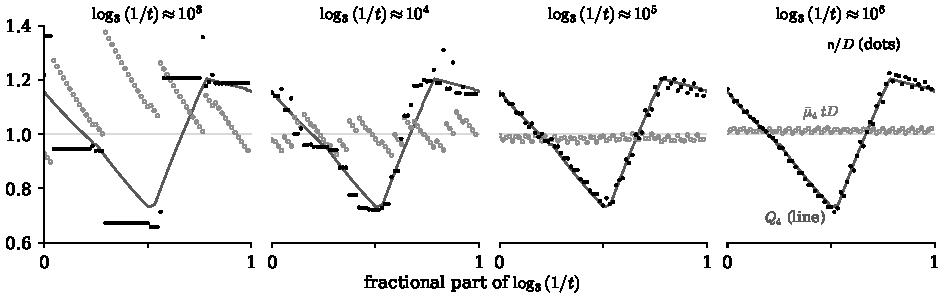
\includegraphics[width=\textwidth]{fig-asymptotics.pdf}
\caption{Both laws for $\cyl_4$. Each panel covers one period of the
threshold, $\log_3(1/t)=10^n+\phi$ with $0\le\phi<1$, sampled at $64$
phases. Open gray dots: $\bar\mu_4tD(t)$. Black dots:
$\ncount(T;t)/D(t)$. Line: the limit $Q_4$ of
Theorem~\ref{thm:periodic}, computed from the actual profiles. At
$10^6$ the largest gap between the dots and the line is $0.030$; both counts approach their limits slowly (see the text).
Floating-point computation (\texttt{fig\_asymptotics.py}); not used in
the proofs.}\label{fig:asym}
\end{figure}

Figure~\ref{fig:asym} shows the two laws directly. It evaluates
$t\,D(t)$ and $t\,\ncount(T;t)$ by the vertex sums of
Corollary~\ref{cor:repr}, with the actual profiles computed from the
secular equation, and $Q_4$ from \eqref{eq:Q}. Terms with $t/m_v<10^{-6}$
are dropped; since $\widehat\xi\le1$ and each path of the walk gains at least $s$ per step, they change $\bar\mu_4t\,\ncount(T;t)$ by less than
$2\cdot10^{-5}$. This bound covers the omitted low-threshold terms,
not the other numerical errors. At $\log_3(1/t)\approx10^3$ only a few depths contribute,
and both ratios jump as the threshold passes individual masses. By
$10^5$ the mass ratio is nearly flat, and the spectral ratio follows
$Q_4$, whose sampled computed range is $[0.731,1.205]$.

The approach is slow and not monotone: at $10^6$, $\bar\mu_4tD$ lies in
$[1.003,1.024]$, further from $1$ than at $10^5$. A heuristic accounts
for this offset. At a given scale, the depths that matter form a window
of standard deviation about $36$ depths at $10^6$. If rule A occurs in
that window with frequency $f$ rather than $1/4$, the local mean step
changes, and $\bar\mu_4tD\approx(1-(f-\frac14)P(k-\frac14)/\bar\mu_4)^{-1}$.
At $10^6$ the window frequency is $0.262$, which predicts $1.0136$; the
observed mean over the period is $1.0137$. The proof needs only that
these window frequencies tend to $1/4$, which is fact~(E). How fast they
do so depends on how well $\alpha$ is approximated by rationals, and
the theorem asserts no rate.

\section{When the law holds: a census of subtree types}\label{sec:positive}

The counterexamples work because the mass count ignores what kind of
subtree each mass carries. This section shows that recording this
information is enough. Suppose $D$ is regularly varying with index $-1$,
the normalized subtree at each vertex is determined by a \emph{type}
taken from a compact space, the profiles depend almost everywhere
continuously on the type, and the types of the vertices of mass above
$s$ have a limiting distribution as $s\downarrow0$. Then
$\ncount(T;t)\sim D(t)$, with no condition on the child ratios
beyond~\eqref{eq:tree}. The tree of continued-fraction cylinders
satisfies these hypotheses, with types ranging over a continuum.

\subsection{A transfer theorem}
\begin{theorem}\label{thm:census}
Assume \eqref{eq:tree}, put $M=M_\theta$, and suppose $D$ is regularly
varying at zero with index $-1$. Let $S$ be a compact metric space, give
each vertex $v$ a type $r_v\in S$, and let
$\xi\colon S\times(0,\infty)\to[0,1]$ be a Borel function with
$\xi(r,u)=0$ for $u\ge M$. Suppose:
\begin{enumerate}
\item[(T1)] $\widehat\xi_v=\xi(r_v,\cdot)$ for every vertex $v$;
\item[(T2)] there is a Borel probability measure $\kappa$ on $S$ such
 that, for every continuous function $f$ on $S$,
 \[
 \frac1{D(s)}\sum_{m_v>s}f(r_v)\longrightarrow\int_Sf\,d\kappa
 \qquad(s\downarrow0);
 \]
\item[(T3)] $\xi$ is continuous at $(\kappa\otimes du)$-almost every
 point of $S\times(0,M)$, and $\int_0^M\xi(r,u)\,du=1$ for
 $\kappa$-almost every $r$.
\end{enumerate}
Then $\ncount(T;t)\sim D(t)$.
\end{theorem}
\begin{proof}
Extend $\xi$ by zero to $S\times[0,M]$. For $t>0$ let $\mu_t$ be the
measure on $S\times[0,M]$ that gives mass $1/D(t)$ to the point
$(r_v,t/m_v)$ for each vertex with $m_v>t/M$. By (F4) and (T1), and
since $\xi(r,u)=0$ for $u\ge M$,
\[
 \frac{\ncount(T;t)}{D(t)}=\int\xi\,d\mu_t .
\]
We first show that $\mu_t$ converges weakly to $\lambda=\kappa\otimes du$.
For continuous $f$ on $S$ and $0<u\le M$, regular variation and (T2) give
\[
 \int f(r)\one_{\{z<u\}}\,d\mu_t(r,z)
 =\frac{D(t/u)}{D(t)}\cdot\frac1{D(t/u)}\sum_{m_v>t/u}f(r_v)
 \longrightarrow u\int_Sf\,d\kappa .
\]
Hence $\int f(r)g(z)\,d\mu_t\to\int f\,d\kappa\int_0^Mg$ for every step
function $g$ on $[0,M]$. The total masses $\mu_t(S\times[0,M])=D(t/M)/D(t)$
are bounded, so the same holds for continuous $g$, by uniform
approximation. Finite sums of such products are uniformly dense in the
continuous functions on $S\times[0,M]$ (Stone--Weierstrass), which
proves the weak convergence.

The function $\xi$ need not be continuous. Let $\xi^*$ and $\xi_*$ be its
upper and lower semicontinuous envelopes. They agree with $\xi$ at its
points of continuity, hence $\lambda$-almost everywhere by (T3); the
slices $z=0$ and $z=M$ are $\lambda$-null. A bounded upper semicontinuous
function on a compact metric space is a decreasing limit of continuous
functions $h_j$. Thus
$\limsup_t\int\xi\,d\mu_t\le\lim_t\int h_j\,d\mu_t=\int h_j\,d\lambda$ for
each $j$, and monotone convergence gives
$\limsup_t\int\xi\,d\mu_t\le\int\xi^*d\lambda=\int\xi\,d\lambda$. The same
argument with $\xi_*$ bounds the limit inferior from below. Finally
$\int\xi\,d\lambda=\int_S\int_0^M\xi(r,u)\,du\,d\kappa(r)=1$ by (T3).
\end{proof}

Theorem~A.4 of~\cite{K26} allows finitely many classes of vertices, with
profiles that converge within each class. Theorem~\ref{thm:census}
allows a continuum of types, but asks that the type determine the
profile exactly.

\emph{The counterexamples fail (T2).} In $\cyl_{r,k}$ the natural type of
a vertex is its phase $\vartheta_{|v|}\in\R/\Z$, which determines its
profile by Lemma~\ref{lem:basic}(4), so (T1) holds. But the census of
phases does not converge. Let $f\ge0$ be continuous on $\R/\Z$ and
$s=e^{-x}$. By Lemma~\ref{lem:walk},
$s\sum_{m_v>s}f(\vartheta_{|v|})=\sum_d\E F_{\vartheta_d}(x-S_d)$ with
$F_\vartheta(u)=f(\vartheta)h(u)$, and the hypotheses of
Theorem~\ref{thm:renewal} hold as in the proof of
Corollary~\ref{cor:D}. Hence
\[
 s\sum_{m_v>s}f(\vartheta_{|v|})
 -\frac P{\bar\mu_{r,k}}\int_0^1f(\vartheta)\,\psi(x/P-\vartheta)\,d\vartheta
 \longrightarrow0,
\]
with $\psi$ as in that proof. The $n$th Fourier coefficient of $\psi$ is
$1/(P+2\pi in)\ne0$, so the limit is independent of $x$ only when $f$ is
constant. Since $sD(s)$ converges, (T2) fails for every nonconstant $f$.

\subsection{Continued fractions}
Every irrational $x\in(0,1)$ has a unique expansion
$x=[0;a_1,a_2,\ldots]$ with positive integer digits. For a finite word
$w=a_1\cdots a_n$ ($n\ge0$), the \emph{cylinder} $I_w$ is the set of
$x$ whose expansion begins with $w$; the empty word gives $(0,1)$. Up to
the countably many rational points, the cylinders $I_{wa}$, $a\ge1$,
partition $I_w$. With Lebesgue measure the cylinders therefore form a
tree of sets as in the Setting, with infinitely many children at every
vertex. Write $T_{\rm CF}$ for its cylinder operator and $D_{\rm CF}$ for
its mass count.

Let $q_{-1}=0$, $q_0=1$ and $q_j=a_jq_{j-1}+q_{j-2}$ be the denominators
of the convergents of $w$, and put $q=q_n$, $p=q_{n-1}$ and $r_w=p/q$.
With the numerators $p_j$ of the convergents, $I_w$ is the image of
$(0,1)$ under $h_w(y)=(p_n+p_{n-1}y)/(q_n+q_{n-1}y)$, and
$|h_w'(y)|=(q+py)^{-2}$ because $p_nq_{n-1}-p_{n-1}q_n=\pm1$;
see~\cite[Chapter~3]{EW}. Moreover $r_w=[0;a_n,\ldots,a_1]$.

\begin{theorem}\label{thm:cf}
The continued-fraction tree satisfies \eqref{eq:tree} with $\theta=\frac12$,
and at every vertex the child with next digit $1$ has between a third
and a half of its parent's length. Its cylinder operator satisfies
\[
 \ncount(T_{\rm CF};t)\sim D_{\rm CF}(t)\sim\frac{6\log2}{\pi^2\,t},
 \qquad
 \lambda_j(T_{\rm CF})\sim\frac{6\log2}{\pi^2\,j}.
\]
The types $r_w$ of the cylinders longer than $s$ are asymptotically
distributed according to the Gauss measure $dr/((1+r)\log2)$ on $[0,1]$.
\end{theorem}

The constant is $1/h$, where $h=\pi^2/(6\log2)$ is the entropy of the
Gauss map~\cite[Section~8.3]{CFV}. The proof uses one lattice-point lemma.

\begin{lemma}\label{lem:coprime}
Let $H$ be a bounded Riemann-integrable function on $[0,C]^2$, extended
by zero. Then, as $R\to\infty$,
\[
 \frac1{R^2}\sum_{\substack{q,p\ge1\\ \gcd(q,p)=1}}H\Big(\frac qR,\frac pR\Big)
 \longrightarrow\frac6{\pi^2}\int H(x,y)\,dx\,dy .
\]
\end{lemma}
\begin{proof}
Write $\one_{\{\gcd(q,p)=1\}}=\sum_{d\mid q,\,d\mid p}\mu(d)$, with $\mu$
the M\"obius function. For fixed $d$, the sum over pairs divisible by $d$,
divided by $R^2$, is a Riemann sum with mesh $d/R$ and tends to
$d^{-2}\int H$. In absolute value it is at most $\norm H_\infty C^2/d^2$ for
all $R$, so the terms with $d>K$ contribute at most
$\norm H_\infty C^2\sum_{d>K}d^{-2}$ uniformly in $R$. Let $R\to\infty$ and
then $K\to\infty$, and use $\sum_d\mu(d)d^{-2}=1/\zeta(2)=6/\pi^2$.
\end{proof}

\begin{proof}[Proof of Theorem~\ref{thm:cf}]
\emph{Masses and types.} The cylinder $I_w$ has length
$m_w=\int_0^1(q+py)^{-2}\,dy=1/(q(q+p))$. Appending a digit $a$ replaces
$(q,p)$ by $(aq+p,q)$, so
\[
 \frac{m_{wa}}{m_w}=\frac{1+r_w}{(a+r_w)(a+1+r_w)},\qquad
 r_{wa}=\frac1{a+r_w}.
\]
The ratio decreases in $a$, and at $a=1$ it equals $1/(2+r_w)\in[\frac13,\frac12]$.
So $\theta=\frac12$ and $M_\theta=2$. Since $m_w\ge t$ forces
$q\le t^{-1/2}$, and only finitely many words have a given $q$, each
$D_{\rm CF}(t)$ is finite. Each rational number in $(0,1)$ has exactly two
finite expansions with positive digits (one ends in a digit at least
$2$, the other in $1$). Since $r_w=[0;a_n,\ldots,a_1]$ and $\gcd(q,p)=1$,
each coprime pair $1\le p<q$ comes from exactly two words, the pair
$(1,1)$ only from the word $1$, and $(1,0)$ only from the empty word.

\emph{The subtree at a vertex depends only on its type.} For $r\in[0,1]$
put $g_r(y)=\sqrt{1+r}/(1+ry)$ on $(0,1)$, so that $\int_0^1g_r^2=1$, and
\[
 A_r=M_{g_r}T_{\rm CF}M_{g_r},\qquad B_r=A_r-R_{g_r},\qquad
 \xi(r,u)=\ncount(A_r;u)-\ncount(B_r;u),
\]
where $M_g$ is multiplication by $g$. The substitution $x=h_w(y)$ turns
the measure $dx/m_w$ on $I_w$ into $g_{r_w}(y)^2\,dy$ and carries $I_{wv}$
to $I_v$. So $Uf=(f\circ h_w)\,g_{r_w}$ is a unitary map from
$L^2(I_w,dx/m_w)$ onto $L^2(0,1)$ with $U\one_{I_{wv}}=g_{r_w}\one_{I_v}$.
Since $R_{gf}=M_gR_fM_g$ for real $g$, $U$ carries $\widehat T_w$ to
$A_{r_w}$ and $\widehat B_w$ to $B_{r_w}$. This is (T1) with $S=[0,1]$.

\emph{Regularity.} The map $r\mapsto g_r$ is uniformly continuous, so
$A_r$ and $B_r$ depend continuously on $r$ in operator norm, and
$B_r=M_{g_r}(T_{\rm CF}-R_\one)M_{g_r}\ge0$. Every rational $r\in[0,1]$ is
a type, so by (F1) and (F3) $\norm{A_r}\le2$, $\xi(r,\cdot)$ takes values
in $\{0,1\}$, vanishes on $[2,\infty)$ and has integral one. By
continuity, $\norm{A_r}\le2$ for every $r$, and $\xi(r,\cdot)\in\{0,1\}$
by rank-one interlacing. For irrational $r$ take rational $r_j\to r$:
off the countably many eigenvalues of $A_r$ and $B_r$ the counts
converge, by Weyl's inequalities, and dominated convergence gives
$\int_0^2\xi(r,u)\,du=1$. The ordered eigenvalues of $A_r$ and $B_r$ are
continuous functions of $r$, again by Weyl's inequalities, so $\xi$ is
Borel. Let $(r,u)$ with $u>0$ lie on none of their graphs, and let
$0<\delta<u/2$ be smaller than the distance from $u$ to the eigenvalues
of $A_r$ and $B_r$. If $r'$ is close enough to $r$ that both operators
move by less than $\delta/2$ in norm, and $|u'-u|<\delta/2$, then no
eigenvalue of $A_{r'}$ or $B_{r'}$ lies between $u$ and $u'$ or on
either, so both counts are constant near $(r,u)$. So the discontinuities of $\xi$ lie on countably many
graphs of continuous functions, a Lebesgue-null set. This proves (T3) for
every $\kappa$ absolutely continuous with respect to $dr$.

\emph{The census.} Let $f$ be continuous on $[0,1]$ and $0<s<\frac12$. By
the count of words,
\[
 \sum_{m_w>s}f(r_w)=f(0)+f(1)+2\!\!\sum_{\substack{1\le p<q,\ \gcd(q,p)=1\\
 q(q+p)<1/s}}\!\!f(p/q).
\]
Apply Lemma~\ref{lem:coprime} with $R=s^{-1/2}$ and
$H(x,y)=f(y/x)\one_{\{0<y<x,\ x(x+y)<1\}}$, which is bounded and
continuous off a null set. The change of variables $r=y/x$,
$u=x(x+y)$ has $dx\,dy=du\,dr/(2(1+r))$, so $\int H=\frac12\int_0^1f(r)\,dr/(1+r)$ and
\[
 s\sum_{m_w>s}f(r_w)\longrightarrow\frac6{\pi^2}\int_0^1\frac{f(r)}{1+r}\,dr .
\]
With $f=1$ this gives $sD_{\rm CF}(s)\to6\log2/\pi^2$; in particular $D_{\rm CF}$ is
regularly varying with index $-1$. Dividing, (T2) holds with $\kappa$ the
Gauss measure. Theorem~\ref{thm:census} gives
$\ncount(T_{\rm CF};t)\sim D_{\rm CF}(t)$. The law for $\lambda_j$ is the
same statement for the inverse function.
\end{proof}

Trees with a single type, such as one that splits every interval in a
fixed non-arithmetic ratio like $3:1$, already have nonvanishing ratios
and obey the law; they are covered by~\cite[Prop.~B.1]{K26}, and also by
Theorem~\ref{thm:census} with one type. The continued-fraction tree adds
a natural example in which the types range over a continuum and every
vertex has infinitely many children. Since Theorem~\ref{thm:main} shows
the law fails for $\cyl_{r,k}$, Theorem~\ref{thm:census} also shows that
no choice of types satisfying (T1) and (T3) for those trees has a
convergent census.

\section{Remarks}\label{sec:remarks}

\emph{Why the earlier transfer theorems do not apply.} The ratio $3/(4L)$
recurs at infinitely many vertices, so the hypothesis of vanishing ratios
fails. The profile theorem of~\cite{K26} needs classes whose counts are
asymptotically proportional to $D$; here the natural classes, rule-A and
rule-B vertices, have masses confined to complementary arcs of the
logarithmic circle, so their counts are not regularly varying. This is
exactly the information that Question~\ref{q:drop}'s hypothesis cannot
see: $D$ records only how many masses lie above $t$, not which kinds of
subtrees they carry. Section~\ref{sec:positive} makes this precise: the
census of types does not converge.

\emph{Other splits.} The base $3$ plays no special role. For an integer
$b\ge2$, let rule A make $L=b^r$ children of relative length
$b/((b+1)L)$ and $L$ of relative length $1/((b+1)L)$, let rule B make
$N=(b+1)b^{k-1}$ equal children, and put $P=\log b$,
$s=\log((b+1)/b)$ and $\alpha=s/P$, which is irrational because $b$ and
$b+1$ are coprime. Every log-length then lies on the grid $ds+P\Z$,
suggesting $\log b$ as the period of a possible limiting law.
Take the rule-A arc to be $[0,a)$ with
$0<a\le\min(\alpha,1-\alpha)$, so that every A depth is followed by a B
depth; for $b=3$ the arc $[0,\frac14)$ qualifies. We expect
Theorem~\ref{thm:main} to hold for every such $b$. The arguments of
Sections~\ref{sec:walk}--\ref{sec:criterion} and
Lemma~\ref{lem:general-error} suggest the same approach, with the
ratio bound $b/(b+1)$ and norm bound $b+1$ replacing $3/4$ and $4$.
Changing the arc also changes the rule frequencies, mean drift, and
Fourier averaging factor; those steps would need to be checked.
For the calculation in Lemma~\ref{lem:nonzero-small}, with
$p=b/(b+1)$ and $q=1/(b+1)$ its limit becomes
$K_b=(1-2pq)z+(2pq)^z-p^z-q^z$ with $z=1+2\pi i/\log b$, and the same
bound gives $\Im K_b\ge(1-2pq)\,2\pi/\log b-(1+2pq)$, which is positive
for $2\le b\le500$ but not for all $b$. We have checked only this
algebra, not a complete proof for other bases.

\emph{The case of non-locked phases.} If the rule at a vertex were chosen
independently of the vertex's logarithmic phase, one expects the same
renewal argument to give a constant limit; we have not checked the
details. The construction uses both an irrational
rotation, to make $D$ smooth, and the identity between the rotation phase
and the logarithmic phase, to make the profile-weighted count periodic.

\emph{Relation to self-similar spectral asymptotics.} Log-periodic
spectral counting functions and their renewal-theoretic treatment are
classical. Kigami--Lapidus~\cite[Thm.~2.4 and Cor.~2.5]{KL} distinguish
whether logarithmic spectral scales lie on a common arithmetic grid
(the \emph{lattice} case) or do not (the \emph{nonlattice} case), for
a class of self-similar fractal Laplacians. Their scales combine weights
from the operator's energy with weights from the measure. Whether those
scales lie on a grid is therefore not a statement about raw cylinder
masses alone. For Sturm--Liouville problems whose weight is
arithmetically self-similar, the eigenvalue count is asymptotically a
power of the eigenvalue times a continuous periodic function of its
logarithm, and
Rastegaev~\cite{Ras} proves that this function is nonconstant for a wide
class of such weights. So a nonconstant periodic leading term is not new
in itself. What is new here is the comparison within one operator: the
unweighted sum of indicator rank-one operators has an eigenvalue count
that oscillates while its own vertex-mass count has a constant leading
term. For continued fractions, the cylinder lengths, their Dirichlet
series and the constant $\pi^2/(6\log2)$ are classical~\cite[Section~8.3]{CFV};
we have not found the eigenvalue law of Theorem~\ref{thm:cf} stated
before. That nonvanishing ratios are compatible with the law was
already known from the stationary trees of~\cite[Prop.~B.1]{K26}.
Naimark and Solomyak~\cite[Example~8.1]{NS} obtain, by the renewal
theorem, an eigenvalue count of the form $\lambda^{-\delta}w(\log(1/\lambda))$
with $w$ periodic, bounded and bounded away from zero, for weighted
Laplacians on homogeneous metric trees. There the operator splits into
one-dimensional problems, nonconstancy of $w$ is not asserted, and no
comparison count is involved. Other tree and ultrametric operators are
studied in~\cite{EHL,LL,BGPW}: exact Weyl-type laws for Hardy operators
on metric trees with edge measures, two-sided entropy bounds for summation
operators, and operators diagonal in a Haar-type basis. We do not claim a
priority result across these different operator classes. The new
counterexamples answer the precise question of~\cite{K26} and show
that no fixed child-ratio bound suffices. The harmonic cancellation
criterion in Theorem~\ref{thm:periodic} is restricted to the family
with the phase-renewal representation used here.

\emph{Zeta functions and complex dimensions.} In the theory of fractal
strings~\cite{LvF}, the poles of the Dirichlet series of the lengths are
called \emph{complex dimensions}, and nonreal poles on the line of
convergence produce log-periodic oscillations in counting functions. For
lattice self-similar strings these poles recur along vertical lines with
a fixed spacing~\cite[Chapters~2--3]{LvF}. Our log-masses also lie on
shifted grids $ds+P\Z$, but the phases $\fr{d\alpha}$ equidistribute,
and Corollary~\ref{cor:zeta} shows that $\zeta_D$ has a nonzero
normalized radial limit on $\Re z=1$ only at $z=1$.
In the vertex formula for $\zeta_T$ each
mass is weighted by $\mathcal M_\vartheta(z)$, which depends on the
phase; this weighting can prevent the cancellation and produce
additional nonzero radial limits for $\zeta_T$.
The radial limits are all we prove; meromorphic
continuation of either series remains open. For the trees
$\cyl_{r,k}$ both series are built from the masses and eigenvalues alone;
no arithmetic zeta function enters. The continued-fraction tree is
different. Writing each pair $q>p\ge1$ as $d$ times a coprime pair
gives, for $\Re z>1$,
\[
 \zeta_D(z)=1+2^{-z}+\frac2{\zeta(2z)}\sum_{q>p\ge1}\frac1{(q(q+p))^z},
\]
where $\zeta$ is the Riemann zeta function. Essentially this series, the
Dirichlet series of the fundamental intervals, is studied
in~\cite[Section~8.3]{CFV}, where its continuation is related to
$\zeta(2z-1)/\zeta(2z)$ and the nontrivial zeros of $\zeta$ enter. The
proof of the vertex formula in Corollary~\ref{cor:zeta} applies to this
tree, and the same rewriting gives $\zeta_T(z)$ with each term weighted
by $z\,\mathcal M_{p/q}(z)$, the Mellin transform of the profile
$\xi(p/q,\cdot)$. Whether $\zeta_T$ continues meromorphically, and whether
it shares the poles of $\zeta_D$, is open.

\emph{Open questions.} (1) Certify or compute the extrema of $Q_k$;
their existence and their role as the endpoints of the limit set are
settled here. (2) Settle $k=2$ in the unreplicated family, and determine
whether a counterexample can have at most two or three children at every
vertex. (3) Theorem~\ref{thm:census} asks that the type determine each
profile exactly, and gives no rate. Find a version with approximate
types, as in~\cite[Thm.~A.4]{K26}, or with an error term.
(4) Determine which limit sets are possible when $D$ is regularly
varying with index $-1$, outside the present periodic family.
(5) Does the law of Theorem~\ref{thm:cf} hold when Lebesgue measure on
$(0,1)$ is replaced by the Gauss measure, or by any continuous positive
density? The masses then depend on where
a cylinder lies, not only on $(q,p)$, so the census needs the positions
and types of cylinders to be equidistributed jointly.

\subsection*{Role of AI}
AI assisted the research development, literature search, proof exposition,
computation and mathematical checking under the author's direction.
Process-separated AI reviews are not independent expert peer review, and no
independent human expert has examined the proofs. The release repository
records the inspected sources, the proof reviews and their dispositions.

\appendix
\section{The interval computation}\label{app:certificate}
The script \texttt{c1\_certificate.py} evaluates $c_1^0$ in interval
arithmetic, which carries rigorous lower and upper bounds through every
operation (\texttt{mpmath.iv}, 40 decimal digits). It
computes $r^{1+i\tau}=r\cos(\tau\log r)+ir\sin(\tau\log r)$ for
$r\in\{\mu_0,\frac34,\mu_1,\frac14\}$ and $\tau=2\pi/\log3$, forms
$(\sum\pm r^{z_1}-1)/z_1$ and multiplies by $(1+i)/(2\pi i)=(1-i)/(2\pi)$. The
output enclosures are
\begin{gather*}
 \Re c_1^0\in[0.09410336970359279,\,0.09410336970359280],\\
 \Im c_1^0\in[0.03826607119219235,\,0.03826607119219236].
\end{gather*}
An independent check by direct numerical quadrature of
$\int\xi^0r^{z_1-1}dr$ and of the $\vartheta$-integrals agrees to $30$
digits. The script also computes $C_N,b_N,E_N$ using interval operations and
asserts the concrete nonvanishing and oscillation-width bounds. For
$N=36$ it gives $E_N<0.08524300$ and
$\pi(|c_1^0|-E_N)>0.0513$; for $N=108$ it gives
$E_N<0.02793825$ and $\pi(|c_1^0|-E_N)>0.2313$.
Only Theorem~\ref{thm:concrete} uses this numerical certificate;
Theorem~\ref{thm:main} uses the elementary nonvanishing argument in
Lemma~\ref{lem:nonzero-small}.

\begin{thebibliography}{99}
\raggedright
\bibitem{ARS}
N.~Arcozzi, R.~Rochberg and E.~Sawyer,
\emph{Carleson measures for analytic Besov spaces},
Rev.\ Mat.\ Iberoamericana \textbf{18} (2002), 443--510.
\href{https://doi.org/10.4171/RMI/326}{doi:10.4171/RMI/326}.

\bibitem{BGPW}
A.~Bendikov, A.~Grigor'yan, Ch.~Pittet and W.~Woess,
\emph{Isotropic Markov semigroups on ultra-metric spaces},
Russian Math.\ Surveys \textbf{69} (2014), 589--680.
\href{https://doi.org/10.1070/RM2014v069n04ABEH004907}{doi:10.1070/RM2014v069n04ABEH004907}.

\bibitem{Bhatia}
R.~Bhatia, \emph{Matrix Analysis}, Graduate Texts in Mathematics 169,
Springer, 1997.

\bibitem{CFV}
J.~Cl\'ement, P.~Flajolet and B.~Vall\'ee,
\emph{Dynamical sources in information theory: a general analysis of
trie structures}, Algorithmica \textbf{29} (2001), 307--369.
\href{https://doi.org/10.1007/BF02679623}{doi:10.1007/BF02679623}.
Section numbers refer to INRIA Research Report 3645 (1999).

\bibitem{EHL}
W.~D.~Evans, D.~J.~Harris and J.~Lang,
\emph{The approximation numbers of Hardy-type operators on trees},
Proc.\ London Math.\ Soc.\ \textbf{83} (2001), 390--418.
\href{https://doi.org/10.1112/plms/83.2.390}{doi:10.1112/plms/83.2.390}.

\bibitem{EW}
M.~Einsiedler and T.~Ward, \emph{Ergodic Theory with a view towards
Number Theory}, Graduate Texts in Mathematics 259, Springer, 2011.

\bibitem{K26}
J.~Kline,
\emph{The eigenvalue decay of the limiting kernel of a sparse Mertens matrix},
version 0.1.0, 2026.
\href{https://doi.org/10.5281/zenodo.23621017}{doi:10.5281/zenodo.23621017}.

\bibitem{KL}
J.~Kigami and M.~L.~Lapidus,
\emph{Weyl's problem for the spectral distribution of Laplacians on
p.c.f.\ self-similar fractals},
Comm.\ Math.\ Phys.\ \textbf{158} (1993), 93--125.
\href{https://doi.org/10.1007/BF02097233}{doi:10.1007/BF02097233}.

\bibitem{LvF}
M.~L.~Lapidus and M.~van Frankenhuijsen,
\emph{Fractal Geometry, Complex Dimensions and Zeta Functions: Geometry
and Spectra of Fractal Strings}, 2nd ed., Springer Monographs in
Mathematics, Springer, New York, 2013.
\href{https://doi.org/10.1007/978-1-4614-2176-4}{doi:10.1007/978-1-4614-2176-4}.

\bibitem{LL}
M.~Lifshits and W.~Linde,
\emph{Compactness properties of weighted summation operators on trees},
Studia Math.\ \textbf{202} (2011), 17--47.
\href{https://doi.org/10.4064/sm202-1-2}{doi:10.4064/sm202-1-2}.

\bibitem{NS}
K.~Naimark and M.~Solomyak,
\emph{Eigenvalue estimates for the weighted Laplacian on metric trees},
Proc.\ London Math.\ Soc.\ (3) \textbf{80} (2000), 690--724.

\bibitem{Petrov}
V.~V.~Petrov, \emph{Sums of Independent Random Variables},
Springer, 1975.

\bibitem{Ras}
N.~V.~Rastegaev,
\emph{On the spectrum of the Sturm--Liouville problem with arithmetically
self-similar weight}, J.\ Spectral Theory \textbf{14} (2024), 1311--1335.
\href{https://doi.org/10.4171/JST/528}{doi:10.4171/JST/528}.

\bibitem{Walters}
P.~Walters, \emph{An Introduction to Ergodic Theory},
Graduate Texts in Mathematics 79, Springer, 1982.
\end{thebibliography}
\end{document}
